%%%%%%%%%%%%%%%%%%%%%%%%%%%%%%%%%%%%%%%%%%%%%%%%%%%%%%%%%%%%%%%
%
% Welcome to Overleaf --- just edit your LaTeX on the left,
% and we'll compile it for you on the right. If you open the
% 'Share' menu, you can invite other users to edit at the same
% time. See www.overleaf.com/learn for more info. Enjoy!
%
%%%%%%%%%%%%%%%%%%%%%%%%%%%%%%%%%%%%%%%%%%%%%%%%%%%%%%%%%%%%%%%
\documentclass[12pt,a4paper,oneside]{book}
\pdfminorversion=7

\let\texendgroup\endgroup

\usepackage[T1]{fontenc}
\usepackage[utf8]{inputenc}
\usepackage[english]{babel}
\usepackage{svg}
\usepackage{amsmath}
\usepackage{amsthm}
\usepackage{amssymb}
\usepackage{tikz}
\usepackage{tcolorbox}
\usepackage{tabularx}
\usetikzlibrary{calc}
\usetikzlibrary{positioning,arrows.meta,fit,backgrounds,shapes.geometric,shapes.misc,chains}
\usepackage[french,ruled,vlined]{algorithm2e}
\usepackage{rotating}
\usepackage{bbding}
\usepackage{cite}
\usepackage{lscape,graphicx}
\usepackage{epstopdf-base}
\usepackage{setspace}
\usepackage{sectsty}
\usepackage{dsfont}
\usepackage{ifpdf}
\usepackage{subfigure}
\usepackage{epsfig}
\usepackage{float}
\usepackage{titlesec}
\usepackage{multibib}
\usepackage{fancyhdr}
\usepackage{lipsum}
\usepackage{soul}
\usepackage[
    a4paper,
    left=1.5cm,
    right=1.5cm,
    top=1.5cm,
    bottom=1.5cm
]{geometry}
%
\renewcommand{\topfraction}{0.9}
\renewcommand{\textfraction}{0.1}
\renewcommand{\floatpagefraction}{0.8}
%

\usepackage{hyperref}


\urlstyle{same}

\setlength{\headheight}{30pt}
\pagestyle{fancy}% \renewcommand{\chaptermark}[1]{\markboth{#1}{}}
\renewcommand{\chaptermark}[1]{\markboth{\MakeUppercase{#1}}{}}
\renewcommand{\sectionmark}[1]{\markright{\MakeUppercase{\thesection.\ #1}}}


%
% \renewcommand{\sectionmark}[1]{\markright{#1}}
%\renewcommand \thesection{\Roman{section}.}
%\renewcommand \thesubsection{\alph{subsection}.}
%
%\newcommand{\helv}{%
%\fontfamily\fontsize{9}{11}\selectfont}

%

% Clear Header Style on the Last Empty Odd pages
\makeatletter
  \def\cleardoublepage{\clearpage\if@twoside \ifodd\c@page\else%
      \hbox{}%
       \thispagestyle{empty}%              % Empty header styles
       \newpage%
       \if@twocolumn\hbox{}\newpage\fi\fi\fi}
\makeatother


\fancyhf{}
\fancyhead[L]{\textit{\nouppercase{\rightmark}}}
\fancyhead[R]{\thepage}

\renewcommand{\headrulewidth}{0pt}
\renewcommand{\footrulewidth}{0pt}
%
\setcounter{secnumdepth}{4}
\setcounter{tocdepth}{4}
%

%
\def\ds{\displaystyle}
\def\dir{./figures}

%


%\setlength\topmargin{0in}
%\setlength\topmargin{0in}
%

%
% Remove page numbering from first page Bibliography
%
%%%%%%%%%%%%%%%%%%%%%%%%% Page de titre %%%%%%%%%%%%%%%%%%%%%%%
\def\baselinestretch{1.5}


\usepackage{listings}
\usepackage{caption}
\usepackage{longtable}
\usepackage{ltcaption}
\usepackage{multirow}
\usepackage{booktabs}

\usepackage{afterpage}

\newcommand\blankpage{%
    \null
    \thispagestyle{empty}%
    \addtocounter{page}{-1}%
    \newpage}


\usepackage[acronym]{glossaries}

\usepackage{lmodern}

\usepackage{arabtex}
\usepackage{utf8}
\setcode{utf8}


\newenvironment{dedication}
  {%\clearpage           % we want a new page          %% I commented this
   \thispagestyle{empty}% no header and footer
   \vspace*{\stretch{1}}% some space at the top
   \itshape             % the text is in italics
   \raggedleft          % flush to the right margin
  }
  {\par % end the paragraph
   \vspace{\stretch{3}} % space at bottom is three times that at the top
   \clearpage           % finish off the page
  }

\newcommand{\reportscreenshot}[4]{%
    \begin{figure}[H]
        \centering
        \IfFileExists{#1}{%
            \includegraphics[width=\textwidth,height=0.72\textheight,keepaspectratio]{#1}%
        }{%
            \fbox{%
                \begin{minipage}[c][0.24\textheight][c]{0.92\textwidth}
                    \centering
                    \textbf{Screenshot to be added}\\[0.8em]
                    #2\\[0.8em]
                    Save the image as:\\[0.3em]
                    \texttt{\detokenize{#1}}
                \end{minipage}%
            }%
        }
        \caption{#3}
        \label{#4}
    \end{figure}%
}

% Legacy package hooks in this template load support files at \begin{document}.
\makeatletter
\def\@fileswithoptions#1{%
        \@ifnextchar[%]
                {\@fileswith@ptions#1}%
                {\@fileswith@ptions#1[]}}
\makeatother


% Legacy package hooks in this template load support files at \begin{document}.
\makeatletter
\def\@fileswithoptions#1{%
    \@ifnextchar[%]
        {\@fileswith@ptions#1}%
        {\@fileswith@ptions#1[]}}
\makeatother

  



% ArabTeX 3.10 leaves one document-level group open under the current MiKTeX
% release. Close it after all package end-document hooks have finished.
\makeatletter
\let\cascade@texend\@@end
\def\@@end{\texendgroup\cascade@texend}
\makeatother

% Keep page numbers in the same top-right position on regular and opening pages.
\fancypagestyle{plain}{%
        \fancyhf{}
        \fancyhead[R]{\thepage}
        \renewcommand{\headrulewidth}{0pt}
        \renewcommand{\footrulewidth}{0pt}}
\fancypagestyle{frontmatterstyle}{%
        \fancyhf{}
        \fancyhead[R]{\thepage}
        \renewcommand{\headrulewidth}{0pt}
        \renewcommand{\footrulewidth}{0pt}}
\renewenvironment{dedication}
    {\thispagestyle{frontmatterstyle}\vspace*{\stretch{1}}\itshape\raggedleft}
    {\par\vspace{\stretch{3}}\clearpage}


%\makenoidxglossaries 

%\newglossaryentry{latex}
%{
       % name=latex,
        %description={Is a mark up language specially suited for scientific documents}
%}



%\selectlanguage{English}



\hypersetup{
    colorlinks=true,
    linkcolor=black,
    filecolor=magenta,      
    urlcolor=cyan,
    pdfauthor={Fares Dkhili},
    pdftitle={STM32Cube Competitor Benchmark},
    pdfsubject={Engineering end-of-studies project report},
    pdfkeywords={STM32Cube, embedded systems, benchmarking, firmware footprint},
    pdfdisplaydoctitle=true,
    pdfpagemode=UseOutlines,
    }



\begin{document}



\definecolor{codegreen}{rgb}{0,0.6,0}
    \definecolor{codegray}{rgb}{0.5,0.5,0.5}
    \definecolor{codepurple}{rgb}{0.58,0,0.82}
    \definecolor{backcolour}{rgb}{0.95,0.95,0.92}
    
    \lstdefinestyle{mystyle}{
        backgroundcolor=\color{backcolour},   
        keywordstyle=\color{magenta},
        numberstyle=\tiny\color{codegreen},
        stringstyle=\color{codepurple},
        basicstyle=\ttfamily\footnotesize,
        breakatwhitespace=false,         
        breaklines=true,                 
        captionpos=b,                    
        keepspaces=true,                 
        numbers=left,                    
        numbersep=5pt,                  
        showspaces=false,                
        showstringspaces=false,
        showtabs=false,                  
        tabsize=2
    }




%\include{Frontmatter/Page_de_garde} %FRENCH ONE

\hypersetup{pageanchor=false}
\include{Frontmatter/Page_de_Garde_EN} % ENGLISH

\afterpage{\blankpage}  %page vide obligatoire

\frontmatter
\hypersetup{pageanchor=true}
\pagestyle{frontmatterstyle}


\input{Frontmatter/Dedication}


\input{Frontmatter/Acknowledgements}


\chapter*{Résumé}
\phantomsection
\addcontentsline{toc}{chapter}{Résumé}

Ce rapport présente un projet de fin d'études réalisé au sein de STMicroelectronics Tunis
afin d'étudier l'écosystème STM32Cube face à des écosystèmes concurrents. Dans une mission
indépendante confiée au stagiaire, nous avons d'abord recherché les cartes STM32 les plus
proches d'une liste de cartes concurrentes fournie par l'équipe d'accueil. Cette étude de
positionnement produit n'a pas déterminé les plateformes des benchmarks ultérieurs. Le
travail expérimental a ensuite commencé par des pilotes USB HID, CDC et MSC comparant STM32
à Renesas et NXP. L'optimisation de la référence STM32 a réduit la RAM et le temps
d'initialisation dans les trois scénarios Renesas. Face à NXP, l'interprétation de la ROM
dépend de l'inclusion du RCC, tandis que MCX-N9 conserve les valeurs rapportées de RAM et
d'initialisation les plus faibles.

Nous avons établi une méthode de benchmarking fondée sur des
fonctionnalités équivalentes, des conditions de compilation documentées, l'empreinte mémoire
extraite des fichiers linker map, des mesures d'exécution lorsqu'elles étaient étayées par
des observations matérielles, ainsi qu'une vérification explicite de l'équivalence sémantique
et de l'équité des comparaisons. Nous avons également conçu deux outils de support~:
\emph{MCU Workflow Studio}, qui structure l'analyse inter-vendeurs des fichiers linker map,
et le \emph{MCU Benchmark Copilot Agent}, qui formalise le processus de création, de portage,
de compilation, de traçabilité et de validation des projets.

La campagne ST--GD32 achevée couvre la pile USB device à travers les scénarios Human
Interface Device (HID) et Communication Device Class (CDC), ainsi que FreeRTOS à travers des
scénarios d'ordonnancement basique, coopératif et préemptif. STM32 nécessite 35--88\,\% de
mémoire flash supplémentaire selon les scénarios, principalement en raison de la couche
Hardware Abstraction Layer (HAL), mais utilise 57--65\,\% de RAM en moins dans les scénarios
USB. Dans les observations rapportées, le temps d'initialisation USB est inférieur de
61,7\,\% sur
STM32, les mesures USB en régime établi sont proches et les mesures FreeRTOS diffèrent au
maximum de 3,3\,\%. Ces résultats nous ont conduits à retenir le module Reset and Clock
Control (RCC) de la HAL et la sélection des fonctionnalités USB à la compilation comme pistes
d'investigation contrôlée, et non comme optimisations déjà démontrées.

La comparaison ST--Texas Instruments associe une analyse statique des pilotes Low-Layer de
STM32CubeC5 et de la bibliothèque de pilotes MSPM33 à douze projets bare-metal appariés
couvrant la conversion analogique-numérique, les entrées-sorties généralistes,
l'I\textsuperscript{2}C, le SPI et l'UART. Sur l'ensemble de ces douze images liées
indépendamment, STM32C5 utilise 2,8\,\% de mémoire flash agrégée supplémentaire et 5,0\,\% de
RAM agrégée en moins. Ces résultats caractérisent la structure du code, la couverture des
Software Development Kits (SDK) et l'empreinte des images complètes. Nous avons ensuite
comparé FreeRTOS à travers des scénarios basique, coopératif et préemptif. Les trois images
STM32C5 utilisent 27,9--29,6\,\% de flash en moins, tandis que MSPM33 économise 56 à 76
octets de RAM. Des observations d'exécution ont également été collectées, mais STM32C5
fonctionne à 144\,MHz contre 32\,MHz pour MSPM33. Après normalisation par la fréquence, le
scénario basique devient presque équivalent; les scénarios coopératif et préemptif restent
affectés par la configuration du noyau et par des primitives de synchronisation différentes.
Ces limites empêchent de conclure globalement sur l'efficacité de l'ordonnanceur.

\noindent\rule[2pt]{\textwidth}{0.5pt}

{\textbf{Mots clés :}}
STM32Cube, benchmarking, empreinte firmware, microcontrôleur, FreeRTOS, USB, GD32, Texas Instruments, pilotes bas niveau, comparaison inter-vendeurs.
\\
\noindent\rule[2pt]{\textwidth}{0.5pt}

% \cleardoublepage
%

\chapter*{Abstract}
\phantomsection
\addcontentsline{toc}{chapter}{Abstract}

This report presents an end-of-studies project carried out at STMicroelectronics Tunis to
study the STM32Cube ecosystem alongside competing microcontroller ecosystems. As an
independent trainee assignment, we first mapped a host-provided list of competitor boards
to their nearest STM32 counterparts; this product study did not determine the later
benchmark platforms. The experimental work then began with USB HID, CDC, and MSC pilots on
STM32 versus Renesas and NXP platforms. Optimising the STM32 reference reduced RAM and
initialisation time in all three Renesas scenarios. In the NXP study, the footprint outcome
depended strongly on whether RCC was included, while MCX-N9 retained lower reported RAM and
initialisation values in the reviewed result tables.

We established a benchmarking method based on matched functionality, documented build
conditions, firmware footprint extracted from linker maps, runtime measurements where
hardware evidence was available, and an explicit review of semantic equivalence and
fairness. We also designed two supporting tools: \emph{MCU Workflow Studio}, which
structures cross-vendor linker-map analysis, and the \emph{MCU Benchmark Copilot Agent},
which encodes the project-creation, porting, build, provenance, and validation workflow.

The completed ST--GD32 campaign covered the USB device stack through Human Interface Device
(HID) and Communication Device Class (CDC) scenarios, and FreeRTOS through basic,
cooperative, and preemptive scheduling scenarios. STM32 required 35--88\,\% more flash across
these scenarios, mainly because of the Hardware Abstraction Layer (HAL), while it used
57--65\,\% less RAM in the USB scenarios. The reported USB initialisation time was
61.7\,\% lower on STM32, steady-state USB measurements were close, and the FreeRTOS
measurements differed by at most 3.3\,\%. These results led us to identify the HAL Reset and
Clock Control (RCC) module and USB compile-time feature selection as targeted areas for
controlled investigation rather than demonstrated optimisations.

The ST--Texas Instruments comparison combined static analysis of the STM32CubeC5 Low-Layer
drivers and the MSPM33 driver library with twelve matched bare-metal projects covering
analog-to-digital conversion, general-purpose input/output, I\textsuperscript{2}C, SPI, and
UART. Across these twelve independently linked images, STM32C5 used 2.8\,\% more aggregate
flash and 5.0\,\% less aggregate RAM. We then compared FreeRTOS through basic, cooperative,
and preemptive scenarios. The three STM32C5 images used 27.9--29.6\,\% less flash, while
MSPM33 used 56--76 fewer RAM bytes. Runtime observations were also collected, but STM32C5
ran at 144\,MHz and MSPM33 at 32\,MHz. The basic result became nearly equal after clock
normalisation; the cooperative and preemptive results remained affected by kernel
configuration and non-equivalent synchronisation primitives. These constraints prevent a
general scheduler-efficiency conclusion from the current measurements.

\noindent\rule[2pt]{\textwidth}{0.5pt}

{\textbf{Key Words:}}
STM32Cube, benchmarking, firmware footprint, microcontroller, FreeRTOS, USB, GD32, Texas Instruments, low-level drivers, cross-vendor comparison.
\\
\noindent\rule[2pt]{\textwidth}{0.5pt}

% \cleardoublepage
%

\chapter*{\RL{ملخص}}
\phantomsection
\addcontentsline{toc}{chapter}{Arabic Abstract}

\setlength{\emergencystretch}{3em}
\begin{RLtext}

\noindent يقدّم هذا التقرير مشروع نهاية الدراسات المنجز بشركة إس تي مايكروإلكترونيكس بتونس.

ويقارن منظومة \LR{STM32Cube} بمنظومات متحكمات دقيقة منافسة. في مهمة مستقلة، زودنا فريق الإشراف بقائمة من لوحات المنافسين وطلب منا تحديد أقرب لوحة \LR{STM32} لكل منها. لم تحدد هذه الدراسة لوحات حملات القياس اللاحقة. بدأ العمل التجريبي بعد ذلك بدراسة \LR{USB HID} و\LR{CDC} و\LR{MSC} على منصات إس تي ورينيساس و\LR{NXP}. خفّض تحسين مشروع إس تي المرجعي استهلاك \LR{RAM} وزمن التهيئة في سيناريوهات رينيساس الثلاثة، بينما ارتبط تفسير نتائج \LR{NXP} بحدود القياس وبإدراج كود \LR{RCC} أو استبعاده.

اعتمدنا وظائف متكافئة وشروط بناء موثقة، واستخرجنا البصمة الذاكرية من ملفات الربط، كما راجعنا التكافؤ الدلالي وعدالة المقارنة.

طوّرنا أداتين مساعدتين: \LR{MCU Workflow Studio} لتنظيم تحليل ملفات الربط بين المصنّعين، و\LR{MCU Benchmark Copilot Agent} لتنظيم إنشاء المشاريع ونقلها وبنائها وتتبع مصادرها والتحقق منها. تساعد الأداتان على توثيق سير العمل، لكن صحة كل نتيجة تبقى مرتبطة بأدلة البناء والقياس والعتاد.

غطّت مقارنة \LR{ST--GD32} سيناريوهات \LR{USB HID} و\LR{CDC} وثلاثة سيناريوهات لـ\LR{FreeRTOS}. استهلك متحكم إس تي ذاكرة فلاش أكثر بنسبة 35--88\%، واستخدم ذاكرة \LR{RAM} أقل بنسبة 57--65\% في سيناريوهات \LR{USB}. أظهرت القياسات المسجلة فرقاً قدره 61,7\% في زمن تهيئة \LR{USB} لصالح إس تي، غير أن غياب العينات المتكررة وحدود القياس المفصلة يمنع تعميم تفسير سببي.

جمعت مقارنة \LR{ST--Texas Instruments} بين تحليل ثابت للمشغلات واثني عشر مشروعاً متناظراً. استخدم متحكم إس تي فلاشاً إجمالياً أكثر بنسبة 2,8\% وذاكرة \LR{RAM} أقل بنسبة 5,0\%. وفي سيناريوهات \LR{Free\-RTOS} الثلاثة، استخدمت صور إس تي فلاشاً أقل بنسبة 27,9--29,6\%، بينما وفّر متحكم \LR{MSPM33} ما بين 56 و76 بايتاً من \LR{RAM}. جُمعت أيضاً قياسات زمن التنفيذ، لكن إس تي عمل بتردد 144 ميغاهرتز مقابل 32 ميغاهرتز لـ\LR{MSPM33}. أصبح السيناريو الأساسي متقارباً بعد التطبيع حسب التردد، في حين بقي تفسير السيناريوهين التعاوني والاستباقي محدوداً باختلاف إعدادات النواة وآليات التزامن. لذلك لا تسمح الأدلة الحالية باستنتاج عام حول كفاءة المجدول أو استهلاك الطاقة.

\end{RLtext}

\noindent\rule[2pt]{\textwidth}{0.5pt}

\begin{RLtext}

{\textbf{الكلمات المفتاحية:}}

\LR{STM32Cube}، قياس الأداء، البصمة الذاكرية، متحكم دقيق، \LR{FreeRTOS}، \LR{USB}، \LR{GD32}، \LR{Texas Instruments}، مقارنة بين المصنّعين.
\\

\end{RLtext}

\noindent\rule[2pt]{\textwidth}{0.5pt}

% \cleardoublepage
%






\tableofcontents
% The table of contents is not listed inside itself.

\cleardoublepage
\phantomsection
\addcontentsline{toc}{chapter}{List of Figures}
\listoffigures

\cleardoublepage
\phantomsection
\addcontentsline{toc}{chapter}{List of Tables}
\listoftables

\cleardoublepage
\phantomsection
\addcontentsline{toc}{chapter}{List of Listings}
\lstlistoflistings

\mainmatter
\pagestyle{fancy}

%debut of chapters

\chapter*{General Introduction}
\phantomsection
\addcontentsline{toc}{chapter}{General Introduction}
\label{chap:cascade-general-introduction}

The internship comprised several related contributions, but not every assignment fed
directly into the benchmark campaigns. The first documented task was an independent board
equivalence search: the host team provided a list of competitor boards and asked us to find
their nearest STM32 counterparts. This product-comparison deliverable did not determine the
boards or scenarios used later in the project.

The experimental work began separately with a pilot Universal Serial Bus (USB) device
campaign on ST, Renesas, and NXP platforms. The pilot combined footprint and initialisation
measurements with an optimisation pass on the STM32 reference projects. It also exposed
repeated manual work in map-file reconciliation, project preparation, and evidence
tracking. We developed MCU Workflow Studio and the MCU Benchmark Copilot Agent in response
to those limitations, then applied the broader methodology in the later GD32 and Texas
Instruments campaigns.

The objective is not to produce a universal vendor ranking. Processor architecture,
memory organisation, clock configuration, compiler output, middleware boundaries, and
scenario design all affect the result. We consequently compare ST with one competing
vendor at a time and restrict each conclusion to the recorded board pair, configuration,
and scenario. Where internal workbook cells disagree with reviewed result images, the
report uses the displayed presentation values and records that source decision explicitly.

Chapter~\ref{chap:general-description} presents the industrial context and requirements.
Chapter~\ref{chap:cascade-board-equivalence} documents the standalone board-equivalence
assignment. Chapter~\ref{chap:cascade-usb-pilot} then begins the independent experimental
work. The two
supporting-tool chapters follow because their requirements emerged from that pilot. The
GD32 and TI chapters then show how the work expanded beyond the initial USB studies, and
the conclusion returns to the limits that govern all of these comparisons.

\input{Cascade/ProjectContextAndRequirements}

\chapter{STM32 Board Equivalence Search}
\label{chap:cascade-board-equivalence}

As a separate assignment during the internship, the host team provided us with a list of
competitor development boards and asked us to identify the nearest STM32 equivalent for
each one. This task was an independent market and product-positioning study. It did not
select the platforms used by the benchmark campaigns presented in the other chapters and
had no direct effect on their scenarios, measurements, or conclusions.

We recorded the outcome in the internal project artifact \emph{board equivalence.pdf}.
The proposed mappings identify the nearest STM32 board according to the characteristics
available for comparison; they are not claims that two boards are interchangeable.

\section{Meaning of board proximity}
\label{sec:cascade-equivalence-method}

For this assignment, \emph{near} means similar according to a combination of product
characteristics. We considered processing class, memory capacity, peripheral support,
development-board capabilities, and intended use. No single candidate matches every
characteristic. Architecture, memory organisation, peripheral implementation, security
features, package, price, and development tooling may remain different.

\section{Candidate mappings}
\label{sec:cascade-equivalence-mappings}

Table~\ref{tab:cascade-board-mappings} records the final candidate mappings in the internal
summary. We retain their status as proposed correspondences and do not attach measurements
to them.

\begin{table}[H]
\centering
\caption{Candidate board mappings recorded in the internal equivalence study. Official product and device sources support the subsequent identifier and lifecycle checks~\cite{nxp-imxrt1060-evk,st-stm32h735g-dk,nxp-frdm-mcxa156,st-nucleo-l552ze-q,renesas-fpb-ra0e1,st-nucleo-l031k6,renesas-fpb-ra8e1,st-nucleo-h743zi2,ti-lp-mspm0c1104,gd32e507-ds,st-nucleo-f429zi}.}
\label{tab:cascade-board-mappings}
\begin{tabular}{lll}
\toprule
Vendor & Candidate board & STM32 candidate \\
\midrule
NXP & MIMXRT1060-EVKC & STM32H735G-DK \\
NXP & FRDM-MCXA156 & NUCLEO-L552ZE-Q \\
Renesas & FPB-RA0E1 & NUCLEO-L031K6 \\
Renesas & FPB-RA8E1 & NUCLEO-H743ZI2 \\
Texas Instruments & LP-MSPM0C1104 & NUCLEO-L031K6 \\
GigaDevice & GD32E507Z-EVAL & NUCLEO-F429ZI \\
\bottomrule
\end{tabular}
\end{table}

The internal summary identifies the first NXP board as MIMXRT1060-EVKC. NXP's current
catalog page is filed under MIMXRT1060-EVKB~\cite{nxp-imxrt1060-evk}; we use it to support
the product-family check, not to assert that the two board revisions are interchangeable.

The source summary spells the first STM32 board as ``SM32H735G-DK''. The official ST
product page confirms that the intended identifier is STM32H735G-DK~\cite{st-stm32h735g-dk}.

\section{Interpretation and limitations}
\label{sec:cascade-equivalence-caveats}

Several mappings cross processor-architecture boundaries. The FPB-RA0E1 and
NUCLEO-L031K6 pair relates Cortex-M23 and Cortex-M0+ platforms; FPB-RA8E1 and
NUCLEO-H743ZI2 relate Cortex-M85 and Cortex-M7 platforms; and GD32E507Z-EVAL and
NUCLEO-F429ZI relate Cortex-M33 and Cortex-M4 platforms. Substantial memory, peripheral,
and software-ecosystem differences may also remain. The mappings should therefore be read
as the result of a nearest-match search within the STM32 portfolio, not as declarations of
technical identity or drop-in compatibility. The current ST product pages also mark the
original NUCLEO-H743ZI and NUCLEO-F429ZI boards obsolete; lifecycle status must therefore
be considered before reusing these historical proposals~\cite{st-nucleo-h743zi2,st-nucleo-f429zi}.

\section{Assignment outcome}
\label{sec:cascade-equivalence-outcome}

The assignment produced six documented competitor-to-STM32 proposals and made the
selection criteria and mismatches explicit. This deliverable was returned to the host team
as a standalone product-comparison study. The work ends at this point; the subsequent USB,
GD32, and TI benchmark campaigns use their own independently selected boards and
experimental controls.

\chapter{Pilot USB Middleware Optimisation and Benchmarking}
\label{chap:cascade-usb-pilot}

The Universal Serial Bus (USB) device stack served as the first experimental test of our
method. We selected Human Interface Device (HID), Communications Device Class (CDC), and
Mass Storage Class (MSC) scenarios because the internal workbook records footprint and
initialisation measurements for all three. The pilot had two objectives: optimise the STM32
reference before comparison and determine which evidence controls were needed for later
campaigns.

\section{Evidence base and validation rules}
\label{sec:cascade-pilot-evidence}

The main Renesas tables use the clearly labelled \emph{Summary} sheet in the supplied pilot
workbook. The \emph{Renesas} sheet provides detailed cross-checks, and
\emph{Initialization Execution time} provides cycle-level traceability for STM32. For the
NXP study, slides~23--25 of the supplied \emph{ST Competitors MW Benchmark} presentation
are the authoritative record because they show the reviewed result tables and scenario
flowcharts. Where those images conflict with workbook cells, we retain the values visible
in the presentation.

The boards for this independent pilot campaign were:
\begin{itemize}
\item Renesas pilot: RA6M5 and STM32H573I-DK;
\item NXP pilot: MCX-N9 and STM32U575.
\end{itemize}
They were selected within the pilot work and are the only platforms to which the results in
this chapter apply.

\section{STM32 baseline-to-optimised results}
\label{sec:cascade-stm32-optimisation}

Table~\ref{tab:cascade-stm32-optimisation} separates the original STM32 USB projects from
their low-footprint configurations. This step prevents avoidable reference-project overhead
from being attributed to the competing platform.

\begin{table}[H]
\centering
\small
\caption{STM32 USB baseline and optimised results from the workbook Summary sheet.}
\label{tab:cascade-stm32-optimisation}
\begin{tabular}{lrrrrrr}
\toprule
& \multicolumn{2}{c}{ROM (bytes)} & \multicolumn{2}{c}{RAM (bytes)} & \multicolumn{2}{c}{Initialisation (ms)} \\
\cmidrule(lr){2-3}\cmidrule(lr){4-5}\cmidrule(lr){6-7}
Scenario & Base & Opt. & Base & Opt. & Base & Opt. \\
\midrule
HID & 54,095 & 52,655 & 43,733 & 36,657 & 0.97 & 0.71 \\
CDC & 33,260 & 33,284 & 18,830 & 17,422 & 0.60 & 0.50 \\
MSC & 70,480 & 70,476 & 108,109 & 69,197 & 2.77 & 2.24 \\
\bottomrule
\end{tabular}
\end{table}

The optimisation does not produce a uniform ROM reduction. CDC increases by 24~bytes and
MSC changes by only 4~bytes. Its stronger effect is visible in RAM and initialisation time,
especially for MSC, whose reported RAM falls from 108,109 to 69,197~bytes. The detailed
initialisation sheet records the corresponding STM32 cycle totals and permits the rounded
times in Table~\ref{tab:cascade-stm32-optimisation} to be traced to the captures.

\section{Optimised STM32 versus Renesas RA6M5}
\label{sec:cascade-pilot-renesas}

\begin{table}[H]
\centering
\small
\caption{RA6M5 and optimised STM32H573I-DK USB results from the workbook Summary sheet.}
\label{tab:cascade-renesas-results}
\begin{tabular}{lrrrrrr}
\toprule
& \multicolumn{2}{c}{ROM (bytes)} & \multicolumn{2}{c}{RAM (bytes)} & \multicolumn{2}{c}{Initialisation (ms)} \\
\cmidrule(lr){2-3}\cmidrule(lr){4-5}\cmidrule(lr){6-7}
Scenario & RA6M5 & STM32 & RA6M5 & STM32 & RA6M5 & STM32 \\
\midrule
HID & 61,380 & 52,655 & 77,896 & 36,657 & 1.59 & 0.71 \\
CDC & 45,224 & 33,284 & 53,090 & 17,422 & 10.98 & 0.50 \\
MSC & 132,712 & 70,476 & 121,252 & 69,197 & 3.84 & 2.24 \\
\bottomrule
\end{tabular}
\end{table}

For these three implementations, the optimised STM32 project has the lower reported ROM,
RAM, and initialisation value in every summary row. The largest timing separation appears
in CDC. The table does not isolate one cause: board choice, generated startup code,
middleware configuration, compiler output, and optimisation decisions remain part of the
measured implementations. The result therefore applies to the recorded RA6M5 and
STM32H573I-DK projects rather than to all Renesas and ST devices.

\section{STM32U575 versus NXP MCX-N9}
\label{sec:cascade-pilot-nxp}

The NXP summary reports two footprint boundaries. Table~\ref{tab:cascade-nxp-with-rcc}
includes the STM32 Reset and Clock Control (RCC) contribution, while
Table~\ref{tab:cascade-nxp-without-rcc} removes it. Presenting both prevents clock setup
from being hidden inside a nominal USB-stack comparison.

\begin{table}[H]
\centering
\small
\caption{STM32U575 and MCX-N9 footprint with STM32 RCC included, as shown in the reviewed presentation.}
\label{tab:cascade-nxp-with-rcc}
\begin{tabular}{lrrrr}
\toprule
& \multicolumn{2}{c}{ROM (bytes)} & \multicolumn{2}{c}{RAM (bytes)} \\
\cmidrule(lr){2-3}\cmidrule(lr){4-5}
Scenario & STM32 & MCX-N9 & STM32 & MCX-N9 \\
\midrule
HID & 16,377 & 13,728 & 2,422 & 1,702 \\
CDC & 17,013 & 13,549 & 3,065 & 1,360 \\
MSC & 35,025 & 26,177 & 13,556 & 11,859 \\
\bottomrule
\end{tabular}
\end{table}

\begin{table}[H]
\centering
\small
\caption{STM32U575 and MCX-N9 footprint with STM32 RCC excluded, as shown in the reviewed presentation.}
\label{tab:cascade-nxp-without-rcc}
\begin{tabular}{lrrrr}
\toprule
& \multicolumn{2}{c}{ROM (bytes)} & \multicolumn{2}{c}{RAM (bytes)} \\
\cmidrule(lr){2-3}\cmidrule(lr){4-5}
Scenario & STM32 & MCX-N9 & STM32 & MCX-N9 \\
\midrule
HID & 11,817 & 12,282 & 2,422 & 1,590 \\
CDC & 12,453 & 12,087 & 3,065 & 1,352 \\
MSC & 27,841 & 24,584 & 13,556 & 11,747 \\
\bottomrule
\end{tabular}
\end{table}

The Summary sheet lists an average STM32 ROM gap of $+26.22\,\%$ with RCC and
$+4.16\,\%$ without RCC. We preserve those reported aggregates rather than infer an
unstated averaging rule. Removing RCC changes the HID ROM ordering, while MCX-N9 retains
the lower reported RAM in all rows. The recorded STM32 RCC ROM contributions are 4,560,
4,560, and 7,184~bytes for HID, CDC, and MSC. The corresponding MCX-N9 clock/configuration
entries are 1,446/112, 1,462/8, and 1,593/112~bytes of ROM/RAM.

\subsection{Initialisation measurements}

\begin{table}[H]
\centering
\small
\caption{STM32U575 and MCX-N9 initialisation times shown in the reviewed presentation.}
\label{tab:cascade-nxp-timing}
\begin{tabular}{lrr}
\toprule
Scenario & STM32U575 (ms) & MCX-N9 (ms) \\
\midrule
HID device & 10 & 5 \\
CDC device & 9.993 & 8.159 \\
MSC host & 112 & 100.03 \\
\bottomrule
\end{tabular}
\end{table}

MCX-N9 has the lower displayed initialisation time in each scenario. The presentation
resolves the workbook's ambiguous MSC label: slide~24 identifies the case as a bare-metal
USB MSC host and shows the measured initialisation path through clock configuration, USB
configuration, and FATFS initialisation before the flash-disk insertion check. We therefore
report it as MSC host initialisation rather than as \texttt{MX\_USB\_Device\_Init()}.

\subsection{Resolution of workbook conflicts}

The workbook contains conflicting alternatives for three footprint entries. The reviewed
presentation resolves them: slide~23 shows 16,377~bytes for STM32 HID ROM and
13,549~bytes for MCX-N9 CDC ROM, while slide~24 shows MSC RAM of 13,556~bytes for
STM32U575 and 11,859~bytes for MCX-N9 with RCC included. The same slide shows
11,747~bytes for MCX-N9 after its clock-configuration RAM is removed. These displayed
values are used in Tables~\ref{tab:cascade-nxp-with-rcc} and
\ref{tab:cascade-nxp-without-rcc}; the contradictory workbook cells are not used.

\section{Pilot synthesis and tool motivation}
\label{sec:cascade-pilot-synthesis}

The pilot established three controls for the later work. We must optimise and document the
reference before comparing it, report the software boundary explicitly, and preserve
conflicts between source artifacts. It also exposed how much repeated effort was required
to classify linker-map content, align projects, and track provenance. Those limitations
became the requirements for MCU Workflow Studio in Chapter~\ref{chap:footprint-tool} and
the MCU Benchmark Copilot Agent in Chapter~\ref{chap:benchmark-agent}.

\input{Cascade/WorkflowStudio}

\input{Cascade/BenchmarkAgent}

\input{Cascade/ExtendedGD32}

\chapter{Benchmarking ST against Texas Instruments}
\label{chap:vs-ti}

\section*{Introduction}

The TI work forms the second extended campaign. It moves beyond the pilot's USB-only scope
and the GD32 campaign by combining source-level driver analysis, matched bare-metal
projects, and FreeRTOS scenarios. Its conclusions must therefore remain separate from the
earlier campaign designs rather than being merged into a single cross-vendor ranking.

Texas Instruments (TI) is one of the world's largest semiconductor manufacturers, with a
broad portfolio of embedded processors and microcontrollers~\cite{ti-about}. Its MSPM0 and
MSPM3 families, built around Arm Cortex-M0+ and Cortex-M33 cores respectively, target
cost-sensitive and mixed-signal applications with a strong emphasis on analog
integration~\cite{ti-mspm33-product}. Unlike GigaDevice, which competes primarily on
pin-compatibility, TI competes on a fundamentally different SDK architecture: a
SysConfig-centric, unified serial peripheral model and a single-layer driver library
(driverlib) rather than the dual HAL/LL approach used by STMicroelectronics.

This chapter presents the ST-versus-TI comparison in two complementary phases. The first is a
comprehensive \textbf{static analysis} of the low-level driver layers of both SDKs. Unlike the
runtime-focused benchmarks in Chapter~\ref{chap:vs-gd32}, this analysis examines source-code
quality and SDK breadth without executing firmware on hardware. The second phase combines
twelve low-level-driver scenarios with a FreeRTOS middleware benchmark covering basic,
cooperative, and preemptive processing. We compare the
STM32CubeC5 Low-Layer (LL) drivers~\cite{stm32cubec5-sw} against the TI MSPM33 SDK
driverlib~\cite{ti-mspm33-sdk} across seven quality dimensions --- lines of code,
documentation coverage, code duplication, cyclomatic complexity, API surface design,
MISRA~C:2012 compliance, and security (CWE analysis). For the scope definition, we also
map the SDK coverage in terms of peripheral drivers, middleware, cryptographic algorithms,
and communication protocols, identifying what each vendor offers exclusively.

All measurements were produced by automated scripts using
\texttt{cloc}~\cite{cloc-tool}, \texttt{cppcheck}~\cite{cppcheck-tool} (with its
\texttt{--addon=misra} and \texttt{--addon=cert} modes),
\texttt{lizard}~\cite{lizard-tool} for cyclomatic complexity, and
\texttt{jscpd}~\cite{jscpd-tool} for duplication detection.

% ====================================================================
\section{Hardware platforms}
\label{sec:ti-boards}

The analysis in this chapter targets driver code for two boards hosting comparable
Cortex-M33 parts. Table~\ref{tab:ti-board-comparison} summarises their key characteristics.

\begin{table}[H]
\centering
\caption{Board and MCU comparison --- STM32C5A3 vs.\ MSPM33C321A~\cite{stm32c5a3-product,stm32-nucleo-c5a3,ti-mspm33-ds,ti-launchpad}.}
\label{tab:ti-board-comparison}
\begin{tabularx}{\textwidth}{@{}l >{\raggedright\arraybackslash}X >{\raggedright\arraybackslash}X@{}}
\toprule
\textbf{Feature} & \textbf{STM32C5A3 (NUCLEO-C5A3ZG)} & \textbf{MSPM33C321A (LP-MSPM33C321A)} \\
\midrule
Core & Arm Cortex-M33 (FPU, DSP, MPU) & Arm Cortex-M33 (FPU, DSP, TrustZone) \\
Max frequency & 144\,MHz & 160\,MHz \\
Flash & 1\,MB (ECC, dual-bank) & 1\,MB (ECC, dual-bank, address swap) \\
SRAM & 256\,KB (128\,KB with ECC) & 256\,KB (ECC) \\
ADC & 3 $\times$ 12-bit, 4.5\,MSPS & 2 $\times$ 12-bit, 9.4\,MSPS \\
DAC & 1 $\times$ 12-bit & 2 $\times$ 8-bit \\
CAN & 2 $\times$ FDCAN & 2 $\times$ CAN\,FD \\
USB & USB\,2.0 FS (Host/Device/DRD) & --- \\
Ethernet & Yes (MAC with DMA) & --- \\
I3C & Yes & --- \\
Debug probe & ST-LINK & XDS110 (EnergyTrace) \\
\bottomrule
\end{tabularx}
\end{table}

Both parts share the same core architecture and identical flash/RAM capacities, which makes
the comparison fair at the silicon level. The STM32C5A3 offers broader connectivity (USB,
Ethernet, I3C), while the MSPM33C321A favours higher analog bandwidth (9.4\,MSPS ADC) and
provides TrustZone support~\cite{ti-mspm33-ds,stm32c5a3-product}.

% ====================================================================
\section{Static analysis of the driver layer}
\label{sec:ti-static-analysis}

This section compares the LL driver layer of STM32CubeC5 against the driverlib of the
MSPM33 SDK. The LL layer was chosen for ST because it is the closest architectural
equivalent to TI's driverlib: both are thin, inline-heavy abstractions over peripheral
registers, designed for performance-critical code. We analyse seven complementary
dimensions.

% --------------------------------------------------------------------
\subsection{Scope and methodology}
\label{subsec:ti-scope}

The analysis targets the following source sets:

\begin{itemize}
  \item \textbf{ST:} all 33 header files in
        \texttt{stm32c5xx\_drivers/ll/} (the LL layer of STM32CubeC5).
  \item \textbf{TI:} all 85 source and header files in
        \texttt{source/ti/driverlib/} and its \texttt{m33/} subdirectory
        (the driverlib of MSPM33 SDK v1.03.00.01).
\end{itemize}

Both sets were analysed on the same workstation under identical tool configurations. The
tools and their roles are:

\begin{itemize}
  \item \textbf{cloc} v2.08~\cite{cloc-tool} --- counts blank, comment, and code lines per
        language and file.
  \item \textbf{lizard}~\cite{lizard-tool} --- computes cyclomatic complexity, number of
        parameters, and token count per function.
  \item \textbf{cppcheck} v2.x~\cite{cppcheck-tool} --- runs MISRA~C:2012 addon
        (\texttt{--addon=misra}) and CWE/CERT checks.
  \item \textbf{jscpd}~\cite{jscpd-tool} --- detects copy-pasted code blocks (duplication).
      \item A custom Python analysis script extracts API surface
        metrics (public/static/inline functions, macros, enums, naming patterns, parameter
        distributions) and documentation coverage (Doxygen blocks, \texttt{@brief},
        \texttt{@param}, \texttt{@return} tags, file headers).
\end{itemize}

% --------------------------------------------------------------------
\subsection{Lines of code}
\label{subsec:ti-loc}

Table~\ref{tab:ti-loc} presents the line-count breakdown for each SDK's driver layer.

\begin{table}[H]
\centering
\caption{Lines-of-code comparison --- ST LL vs.\ TI driverlib.}
\label{tab:ti-loc}
\begin{tabular}{l r r}
\toprule
\textbf{Metric} & \textbf{ST (LL)} & \textbf{TI (driverlib)} \\
\midrule
Source files      &        33 &        85 \\
Blank lines       &     5\,744 &     8\,747 \\
Comment lines     &    57\,649 &    45\,763 \\
Code lines        &    22\,292 &    27\,972 \\
\midrule
Total lines       &    85\,685 &    82\,482 \\
Comment-to-code ratio & 2.59 & 1.64 \\
\bottomrule
\end{tabular}
\end{table}

ST delivers its LL layer in 33 header-only files containing 22\,292 lines of code, while
TI spreads its driverlib across 85 files (both \texttt{.c} and \texttt{.h}) with
27\,972 code lines. Despite having 25\% more code, TI's total line count is slightly
lower because ST invests significantly more in inline comments: 57\,649 comment lines
versus 45\,763, yielding a comment-to-code ratio of 2.59 for ST compared with 1.64 for TI.
This difference reflects ST's header-only, fully-documented inline function strategy, where
each function carries extensive Doxygen annotations embedded alongside the implementation.

% --------------------------------------------------------------------
\subsection{Documentation coverage}
\label{subsec:ti-doc}

We measured documentation quality through Doxygen tag extraction.
Table~\ref{tab:ti-doc} summarises the results.

\begin{table}[H]
\centering
\caption{Documentation coverage --- ST LL vs.\ TI driverlib.}
\label{tab:ti-doc}
\begin{tabular}{l r r}
\toprule
\textbf{Metric} & \textbf{ST (LL)} & \textbf{TI (driverlib)} \\
\midrule
Total functions         &   3\,713 &   3\,056 \\
Documented functions    &   3\,613 &   2\,525 \\
\textbf{Doc.\ coverage} & \textbf{97.3\,\%} & \textbf{82.6\,\%} \\
\midrule
Doxygen blocks          &   5\,967 &   3\,357 \\
\texttt{@brief} tags    &   3\,826 &   5\,568 \\
\texttt{@param} tags    &   4\,440 &   3\,970 \\
\texttt{@return} tags   &   1\,705 &   2\,172 \\
File headers            &      33  &      85  \\
Inline comments         &       0  &     283  \\
\bottomrule
\end{tabular}
\end{table}

ST achieves 97.3\% function-level documentation coverage, leaving only 100 undocumented
functions. TI reaches 82.6\%, with 531 undocumented functions --- mostly in \texttt{.c}
implementation files, where TI concentrates complex logic (e.g.\ flash controller
operations, PLL configuration) without per-function Doxygen blocks. This architectural
choice is deliberate: TI documents the \emph{header} API thoroughly but omits Doxygen in
\texttt{.c} bodies, whereas ST's header-only approach means every function definition is
also its documented declaration.

Interestingly, TI uses more \texttt{@brief} tags (5\,568 vs.\ 3\,826) and more
\texttt{@return} tags (2\,172 vs.\ 1\,705), suggesting that when TI does document a
function, it tends to be descriptive about purpose and return values. ST, however, produces
78\% more Doxygen blocks overall (5\,967 vs.\ 3\,357), reflecting its higher raw volume of
documented entities.

% --------------------------------------------------------------------
\subsection{Code duplication}
\label{subsec:ti-dup}

Table~\ref{tab:ti-dup} presents the duplication metrics.

\begin{table}[H]
\centering
\caption{Code duplication --- ST LL vs.\ TI driverlib.}
\label{tab:ti-dup}
\begin{tabular}{l r r}
\toprule
\textbf{Metric} & \textbf{ST (LL)} & \textbf{TI (driverlib)} \\
\midrule
Total lines analysed     &    85\,685 &    82\,403 \\
Code lines               &    10\,461 &    18\,008 \\
Duplicate blocks         &        71 &       414 \\
Duplicate lines          &       229 &     1\,306 \\
\textbf{Duplication \%}  & \textbf{2.19\,\%} & \textbf{7.25\,\%} \\
\midrule
Same-file clones         &        71 &       338 \\
Cross-file clones        &         0 &        76 \\
\bottomrule
\end{tabular}
\end{table}

TI's driver layer exhibits 3.3$\times$ more duplication than ST's (7.25\% vs.\ 2.19\%).
All 71 duplicate blocks in ST occur within the same file, typically in symmetric
getter/setter pairs for multi-channel peripherals (e.g.\ ADC rank configuration).
TI, by contrast, has 76 cross-file clones --- code that is structurally identical across
different peripheral modules. This pattern arises from TI's UniComm architecture, where
\texttt{dl\_unicommuart.h}, \texttt{dl\_unicommspi.h}, and \texttt{dl\_unicommi2cc.h}
share a common General Serial Controller (GSC) base but replicate similar interrupt-handling
and configuration boilerplate in each specialisation.

The higher duplication in TI is not inherently a quality defect --- it reflects a design
choice that trades some code reuse for peripheral-specific readability. However, from a
maintenance perspective, ST's lower duplication means fewer locations to update when fixing
a bug or adapting to silicon errata.

% --------------------------------------------------------------------
\subsection{Cyclomatic complexity}
\label{subsec:ti-complexity}

Cyclomatic complexity (CC) measures the number of linearly independent paths through a
function; higher values indicate more decision branches and, consequently, harder-to-test
code~\cite{lizard-tool}. We ran Lizard on every function in both driver sets and
summarise the results in Table~\ref{tab:ti-complexity}.

\begin{table}[H]
\centering
\caption{Cyclomatic complexity comparison --- ST LL vs.\ TI driverlib.}
\label{tab:ti-complexity}
\begin{tabular}{l r r}
\toprule
\textbf{Metric} & \textbf{ST (LL)} & \textbf{TI (driverlib)} \\
\midrule
Analysed functions       &    3\,542 &    2\,539 \\
Mean CC                  &      4.44 &      7.35 \\
Median CC                &         4 &         5 \\
Maximum CC               &        49 &       141 \\
\midrule
Functions with CC $>$ 10 &    44 \scriptsize(1.2\,\%) &   335 \scriptsize(13.2\,\%) \\
Functions with CC $>$ 20 &    12 \scriptsize(0.3\,\%) &    97 \scriptsize(3.8\,\%) \\
\bottomrule
\end{tabular}
\end{table}

Under the study's declared CC\,=\,10 review threshold, ST's analysed driver code is
flatter: the average function has fewer than five decision points, and 1.2\,\% of functions
exceed that threshold. The maximum (CC\,=\,49) occurs in a temperature-calculation
helper (\texttt{LL\_ADC\_CALC\_TEMPERATURE}) that contains a long chain of calibration
look-ups.

TI's SDK shows a heavier tail: 13.2\,\% of its functions exceed CC\,=\,10, with a peak of
141 in a single function. Many of these high-complexity functions reside in the UniComm
serial-controller layer, where a large \texttt{switch} dispatches configuration variants
for UART, SPI, and I\textsuperscript{2}C through a shared code path. While this design
consolidates peripheral logic, it concentrates branching in ways that complicate unit testing
and formal verification.

Under this metric, ST's analysed source set contains fewer functions above the declared
review threshold. The result does not by itself establish maintainability or safety.

% --------------------------------------------------------------------
\subsection{API surface}
\label{subsec:ti-api}

Table~\ref{tab:ti-api} compares the API design characteristics.

\begin{table}[H]
\centering
\caption{API surface comparison --- ST LL vs.\ TI driverlib.}
\label{tab:ti-api}
\begin{tabular}{l r r}
\toprule
\textbf{Metric} & \textbf{ST (LL)} & \textbf{TI (driverlib)} \\
\midrule
Public functions         &    3\,543 &    2\,500 \\
Static functions         &         1 &        42 \\
Inline functions         &    3\,543 &    2\,032 \\
Functional macros        &       194 &        27 \\
Constant macros          &     3\,993 &    3\,271 \\
Enums                    &         1 &       361 \\
Typedefs                 &         0 &       470 \\
\midrule
Avg.\ parameters/func.  &      1.17 &      1.69 \\
Max parameters           &         8 &         8 \\
\texttt{extern "C"} guards &    33 &        43 \\
Include guards           &        33 &         0 \\
\bottomrule
\end{tabular}
\end{table}

The two APIs reflect fundamentally different design philosophies:

\begin{itemize}
  \item \textbf{ST LL} exposes 3\,543 public functions, \emph{all} of which are
        \texttt{\_\_STATIC\_INLINE}. The API is almost entirely composed of one-parameter
      getters and status queries.
        Type safety relies on constant macros rather than enums. The naming convention
        follows the \texttt{LL\_PERIPHERAL\_Action} pattern consistently across all 33
        files.
  \item \textbf{TI driverlib} exposes 2\,500 public functions, of which 2\,032 are inline
        (81\%). It makes heavier use of enums (361 enum types) and typedefs (470) for
        configuration parameters, which improves type safety and IDE autocompletion at the
        cost of a more complex type graph. The naming convention follows
        \texttt{DL\_Peripheral\_Action} uniformly. Functions tend to take more parameters
        on average (1.69 vs.\ 1.17), reflecting a more configuration-object-oriented
        style where a single call sets multiple related fields.
\end{itemize}

ST's 194 functional macros versus TI's 27 show that the analysed ST source set uses more
preprocessor computation in places such as register-offset calculations and bit-field
assembly. Inline functions permit stronger compile-time type checking than function-like
macros, but this study did not compare generated machine code or debugging productivity.

% --------------------------------------------------------------------
\subsection{MISRA~C:2012 static-analysis findings}
\label{subsec:ti-misra}

Both SDKs were analysed using \texttt{cppcheck} with the MISRA~C:2012
addon~\cite{misra-c2012}. Table~\ref{tab:ti-misra} presents the per-rule breakdown.

\begin{table}[H]
\centering
\caption{Cppcheck MISRA-addon findings --- ST LL vs.\ TI driverlib.}
\label{tab:ti-misra}
\begin{tabular}{l l r r}
\toprule
\textbf{Rule} & \textbf{Description} & \textbf{ST} & \textbf{TI} \\
\midrule
17.3 & Function declared implicitly       & 3\,541 &  281 \\
11.4 & Conversion between pointer and integer & 84 &    4 \\
10.6 & Composite expression assigned to wider type & 29 & --- \\
20.7 & Macro parameter not enclosed in parentheses & 21 & --- \\
7.3  & Lower-case ``l'' suffix on literal  &    18 & --- \\
10.4 & Incompatible essential types in operation & --- & 67 \\
12.1 & Precedence of operators unclear     & --- &   52 \\
18.4 & Pointer arithmetic                  & --- &   76 \\
15.5 & Multiple return statements          &     4 &   14 \\
10.1 & Operands of inappropriate essential type & --- & 13 \\
3.1  & Comment contains nested comment     & --- &   11 \\
Other & Various minor rules                &    6 &   33 \\
\midrule
\textbf{Total} & & \textbf{3\,703} & \textbf{551} \\
\bottomrule
\end{tabular}
\end{table}

\subsubsection*{Interpretation}
The raw Cppcheck output reports 3\,703 findings for ST and 551 for TI. Rule~17.3 accounts
for 3\,541 ST findings and 281 TI findings. The current analysis attributes many ST
findings to processing header-only inline code in isolation, but the original preprocessing
inputs and a compilation-database rerun are not available with the report artifacts. We
therefore present exclusion of Rule~17.3 only as a sensitivity calculation, not as proof
that every such finding is a false positive. Under that exclusion, the counts are 162 for
ST and 270 for TI. These are tool-reported findings for the analysed source sets and do not
constitute MISRA certification or a complete compliance assessment.

The remaining findings also require source-level review. Rule~11.4 includes casts between
integers and peripheral base-address pointers, a common low-level-driver pattern, while TI's
reported findings span rules concerning pointer arithmetic, essential types, and operator
precedence. Counts alone do not establish the severity or correctness impact of these
patterns.

\subsubsection*{Security analysis (CWE)}
Both driver layers returned \textbf{zero CWE findings} from \texttt{cppcheck}'s CERT/CWE
checker. Neither SDK contains patterns flagged as common weakness enumerations, which is
expected for thin, register-level driver code that performs no dynamic allocation, string
handling, or network I/O.

% ====================================================================
\section{SDK coverage comparison}
\label{sec:ti-sdk-coverage}

Beyond driver-layer quality, the breadth of a selected SDK release --- how many peripherals, middleware
stacks, and communication protocols it supports out of the box --- determines the
development effort required for a real product. We inventoried the selected STM32CubeC5
and MSPM33 SDK source sets file by file and identified features present on only one side
within those releases~\cite{stm32cubec5-sw,ti-mspm33-sdk}.

% --------------------------------------------------------------------
\subsection{Peripheral driver coverage}
\label{subsec:ti-periph-gaps}

Table~\ref{tab:ti-periph-exclusive} lists the peripheral drivers present in only one
SDK.\footnote{For brevity, only a representative subset of ST's 25 exclusive drivers is
shown; the full list is available in the analysis output.}

\begin{table}[H]
\centering
\caption{Exclusive peripheral drivers in the selected SDK releases~\cite{stm32cubec5-sw,ti-mspm33-sdk}.}
\label{tab:ti-periph-exclusive}
\begin{tabular}{l p{5.5cm} l}
\toprule
\textbf{Vendor} & \textbf{Driver} & \textbf{Capability} \\
\midrule
\multicolumn{3}{l}{\textit{ST-exclusive (25 drivers)}} \\
ST & CORDIC accelerator              & HW trigonometric/hyperbolic math \\
ST & DAC (12-bit)                    & Full DAC peripheral \\
ST & Ethernet MAC                    & On-chip networking \\
ST & USB Host / Device / DRD         & Full USB stack support \\
ST & I3C controller                  & Next-gen I3C bus \\
ST & HASH accelerator (SHA)          & HW SHA-1/SHA-256 \\
ST & OPAMP                           & On-chip operational amplifier \\
ST & ICACHE controller               & Configurable instruction cache \\
ST & XSPI (Octo/Quad-SPI)           & Advanced memory-mapped SPI \\
ST & LPUART, USART, SmartCard, SMBus & Extended serial protocols \\
\midrule
\multicolumn{3}{l}{\textit{TI-exclusive (16 drivers)}} \\
TI & High-Speed ADC (HSADC)          & Dedicated 9.4\,MSPS ADC block \\
TI & General Serial Controller (GSC) & Unified serial engine \\
TI & UniComm (I2C/SPI/UART)          & Configurable serial block \\
TI & Signal Processing Subsystem     & On-chip analog processing \\
TI & Low-Frequency Subsystem (LFSS)  & Unified RTC + tamper + scratchpad \\
TI & Key Store Controller            & HW key management \\
TI & Error Action Module             & HW automatic fault handling \\
TI & UART extend (IrDA, Manchester)  & Extended UART modes \\
\bottomrule
\end{tabular}
\end{table}

ST leads with 25 exclusive peripheral drivers to TI's 16. The most significant gaps are
in connectivity: ST offers USB, Ethernet, and I3C, which are entirely absent from the
MSPM33C321A. TI compensates with stronger analog integration (high-speed ADC, signal
processing subsystem) and a unified serial architecture that consolidates UART, SPI, and
I2C into a single configurable peripheral.

% --------------------------------------------------------------------
\subsection{Middleware coverage}
\label{subsec:ti-mw-gaps}

Table~\ref{tab:ti-mw-exclusive} compares the middleware stacks.

\begin{table}[H]
\centering
\caption{Exclusive middleware in the selected SDK releases~\cite{stm32cubec5-sw,ti-mspm33-sdk}.}
\label{tab:ti-mw-exclusive}
\begin{tabular}{l l p{6cm}}
\toprule
\textbf{Vendor} & \textbf{Middleware} & \textbf{Purpose} \\
\midrule
ST & FileX              & FAT-compatible embedded file system \\
ST & LevelX             & Flash wear-leveling (NAND/NOR) \\
ST & LwIP               & Lightweight TCP/IP stack \\
ST & USBX               & USB device/host class drivers \\
ST & mbedTLS             & TLS/SSL library (TLS~1.2/1.3) \\
ST & Open Bootloader     & Multi-interface bootloader \\
ST & stFCF               & Security provisioning framework \\
ST & stCryptoLib          & Comprehensive crypto library \\
\midrule
TI & Edge AI             & On-device ML inference \\
TI & LVGL                & Embedded graphics/GUI library \\
TI & LIN Bus             & Automotive LIN protocol \\
TI & DALI                & Smart lighting protocol \\
TI & IQmath              & Fixed-point DSP math library \\
TI & Post-Quantum Crypto & ML-DSA (Dilithium) signatures \\
TI & Curve25519          & Modern elliptic curve crypto \\
\bottomrule
\end{tabular}
\end{table}

ST provides 8 exclusive middleware components focused on connectivity (USB, Ethernet/IP,
file system) and security (TLS, crypto library, secure boot). TI provides 7 exclusive
components that target emerging domains: Edge~AI for on-device machine learning, LVGL for
embedded GUIs, automotive protocols (LIN, DALI), and forward-looking cryptography
(post-quantum ML-DSA, Curve25519).

% --------------------------------------------------------------------
\subsection{Cryptographic algorithm coverage}
\label{subsec:ti-crypto}

Table~\ref{tab:ti-crypto} provides a detailed comparison of the algorithms available in
each vendor's crypto libraries.

\begin{table}[H]
\centering
\caption{Cryptographic algorithm inventory for the selected SDK releases~\cite{stm32cubec5-sw,ti-mspm33-sdk}.}
\label{tab:ti-crypto}
\begin{tabular}{l c c}
\toprule
\textbf{Algorithm} & \textbf{ST (stCryptoLib)} & \textbf{TI (crypto/)} \\
\midrule
AES (ECB, CBC, CTR, GCM)  & \checkmark & \checkmark \\
AES-CCM / AES-XTS         & \checkmark & ---        \\
SHA-224/256                & \checkmark & \checkmark \\
SHA-384/512, SHA-3         & \checkmark & ---        \\
HMAC                       & \checkmark & \checkmark \\
CMAC / KMAC                & \checkmark & ---        \\
RSA (PKCS\#1)              & \checkmark & \checkmark \\
ECDSA / ECDH               & \checkmark & \checkmark \\
EdDSA (Ed25519)            & \checkmark & \checkmark \\
SM2 / SM3 (Chinese std.)   & \checkmark & ---        \\
ChaCha20-Poly1305          & \checkmark & ---        \\
ML-DSA (Post-Quantum)      & ---        & \checkmark \\
Curve25519 / X25519         & ---        & \checkmark \\
TRNG (HW)                  & \checkmark & \checkmark \\
PKA (HW)                   & \checkmark & \checkmark \\
Key Store (HW)              & \checkmark & \checkmark \\
\bottomrule
\end{tabular}
\end{table}

ST offers the broader algorithm portfolio (10+ exclusive algorithms), covering legacy
standards (SHA-1), Chinese national standards (SM2/SM3), and authenticated-encryption
modes (AES-CCM, ChaCha20-Poly1305). TI, while narrower, holds a forward-looking advantage
with post-quantum cryptography (ML-DSA/Dilithium) and modern elliptic-curve primitives
(Curve25519), which positions it well for long-term security requirements~\cite{nist-pqc}.

% --------------------------------------------------------------------
\subsection{Communication protocol coverage}
\label{subsec:ti-comm}

Table~\ref{tab:ti-comm-protocols} summarises the communication protocol support.

\begin{table}[H]
\centering
\caption{Communication protocol inventory for the selected SDK releases~\cite{stm32cubec5-sw,ti-mspm33-sdk}.}
\label{tab:ti-comm-protocols}
\begin{tabular}{l c c}
\toprule
\textbf{Protocol} & \textbf{ST} & \textbf{TI} \\
\midrule
UART / SPI / I2C / I2S / CAN\,FD   & \checkmark & \checkmark \\
USB (Device + Host)                  & \checkmark & ---        \\
Ethernet                             & \checkmark & ---        \\
I3C                                  & \checkmark & ---        \\
SMBus / SmartCard (ISO~7816)         & \checkmark & ---        \\
LPUART / USART (synchronous)         & \checkmark & ---        \\
IrDA mode / Manchester encoding      & ---        & \checkmark \\
LIN Bus                              & ---        & \checkmark \\
\bottomrule
\end{tabular}
\end{table}

ST supports 7 exclusive communication protocols, with USB and Ethernet being the most
impactful for connected applications. TI brings 3 exclusive capabilities: IrDA mode,
Manchester encoding (both through its extended UART), and LIN Bus for automotive
applications.

% ====================================================================
\section{Static-analysis summary}
\label{sec:ti-static-summary}

Table~\ref{tab:ti-summary-scoreboard} provides a consolidated view of the static-analysis
results.

\begin{table}[H]
\centering
\caption{Static-analysis scoreboard --- STM32CubeC5 LL vs.\ TI MSPM33 driverlib.}
\label{tab:ti-summary-scoreboard}
\small
\begin{tabularx}{\textwidth}{@{}>{\raggedright\arraybackslash}X r r >{\raggedright\arraybackslash}p{3.2cm}@{}}
\toprule
\textbf{Dimension} & \textbf{ST result} & \textbf{TI result} & \textbf{Advantage} \\
\midrule
Code lines            & 22\,292          & 27\,972          & ST (leaner) \\
Documentation coverage & 97.3\,\%        & 82.6\,\%         & ST \\
Code duplication       & 2.19\,\%        & 7.25\,\%         & ST \\
Cyclomatic complexity  & 4.44 avg        & 7.35 avg         & ST (flatter) \\
API functions          & 3\,543          & 2\,500           & ST (wider) \\
Type safety (enums)    & 1               & 361              & TI \\
MISRA-addon findings excluding Rule~17.3 & 162\textsuperscript{*} & 270 & Sensitivity only \\
Security (CWE)         & 0               & 0                & Tie \\
Exclusive peripherals  & 25              & 16               & ST \\
Exclusive middleware   & 8               & 7                & Balanced \\
Crypto algorithms      & 10+ exclusive   & 2 exclusive      & ST (breadth), TI (PQC) \\
Comm.\ protocols       & 7 exclusive     & 3 exclusive      & ST \\
\bottomrule
\end{tabularx}
\par\smallskip
{\footnotesize \textsuperscript{*}Sensitivity calculation; Rule~17.3 findings were not individually adjudicated.}
\end{table}

Within the analysed source sets, ST's LL driver layer contains fewer code lines, higher
measured documentation coverage, less measured duplication, and a lower adjusted
MISRA-addon finding count when Rule~17.3 is excluded as a sensitivity calculation. The SDK
inventory also records broader ST coverage in several connectivity and security categories.

TI, however, brings distinct strengths: stronger type safety through enums and typedefs,
forward-looking post-quantum cryptography, superior analog integration (9.4\,MSPS ADC), a
unified serial architecture that simplifies board design, and emerging-domain middleware
(Edge~AI, LVGL, automotive protocols). These advantages position TI well for mixed-signal
and AI-at-the-edge applications where connectivity is less critical than analog performance.
% ====================================================================
\section{Functional analysis of the driver layer}
\label{sec:ti-functional-analysis}

Static metrics describe the structure of the two driver libraries, but they do not establish
whether equivalent application behaviours can be exercised in practice. We therefore prepared
twelve bare-metal scenarios that pair TI driverlib examples with STM32CubeC5 LL examples. The
scenarios cover conversion, GPIO control, I\textsuperscript{2}C, SPI, and UART behaviours, as
summarised in Table~\ref{tab:ti-functional-scenarios}. They constitute the first part of the
functional phase; the second part applies the same process to the FreeRTOS middleware stack.

\subsection{Benchmark design and observables}
\label{subsec:ti-functional-design}

Each scenario starts in \texttt{main()}, configures the relevant peripheral through the vendor's
low-level API, triggers an observable operation, and verifies completion. The TI examples are
drawn from the MSPM33 SDK~\cite{ti-mspm33-sdk}, while the ST counterparts use the
STM32CubeC5 LL example set~\cite{stm32cubec5-sw}. The examples are
bare-metal applications: no RTOS scheduling or middleware service is included in the measured
scope. For serial transfers, the controller/master side initiates communication and the
target/responder or peripheral/slave side completes the paired exchange. Completion is exposed
through a peripheral flag or interrupt, a byte-for-byte buffer comparison, an LED state, a
debugger-visible value, or a UART output.

\begin{figure}[H]
\centering
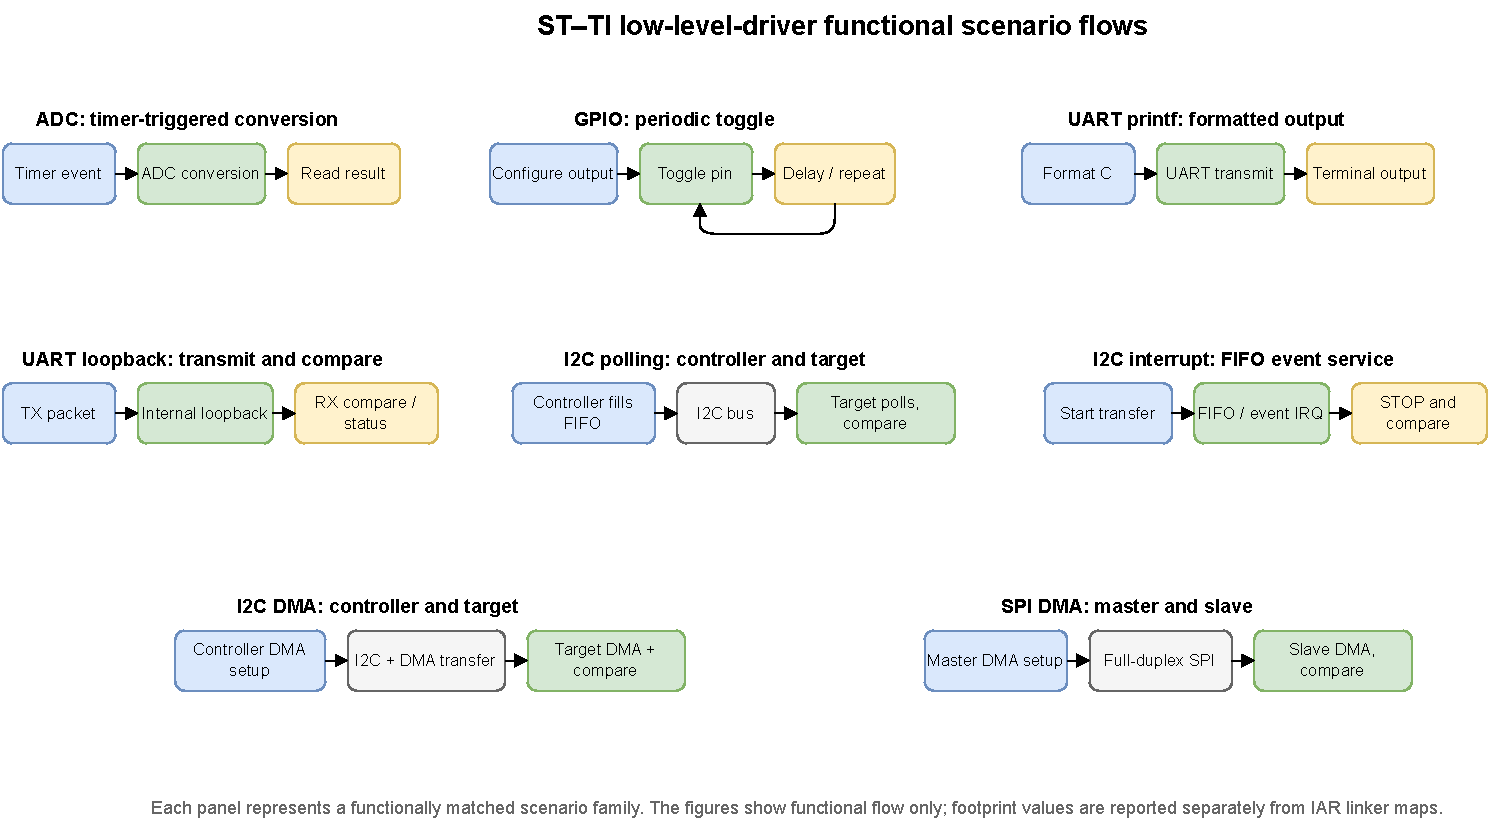
\includegraphics[width=\textwidth]{Figures/ti-functional/scenario-flows.pdf}
\caption{Functional flows of the eight low-level-driver scenario families. I\textsuperscript{2}C and SPI panels represent their paired controller/target and master/slave projects, respectively; the flows define functional behaviour and not a timing window.}
\label{fig:ti-functional-scenario-flows}
\end{figure}

\begin{table}[H]
\centering
\small
\caption{ST--TI low-level-driver functional scenario mapping.}
\label{tab:ti-functional-scenarios}
\begin{tabularx}{\textwidth}{c l X X}
\toprule
\textbf{ID} & \textbf{Scenario} & \textbf{TI driverlib example} & \textbf{STM32CubeC5 LL example} \\
\midrule
1 & ADC, timer-triggered conversion & ADC single conversion & ADC single conversion \\
2 & GPIO output toggle & GPIO I/O toggling & GPIO toggle \\
3 & I\textsuperscript{2}C controller transmit, DMA & I2C two-board DMA, controller & I2C DMA, controller \\
4 & I\textsuperscript{2}C target receive, DMA & I2C two-board DMA, target & I2C DMA, responder \\
5 & I\textsuperscript{2}C controller transmit, interrupt & I2C two-board interrupt, controller & I2C interrupt, controller \\
6 & I\textsuperscript{2}C target receive, interrupt & I2C two-board interrupt, target & I2C interrupt, responder \\
7 & I\textsuperscript{2}C controller transmit, polling & I2C two-board polling, controller & I2C polling, controller \\
8 & I\textsuperscript{2}C target receive, polling & I2C two-board polling, target & I2C polling, responder \\
9 & SPI controller/master full-duplex, DMA & SPI two-board DMA, controller & SPI DMA, master \\
10 & SPI peripheral/slave full-duplex, DMA & SPI two-board DMA, peripheral & SPI DMA, slave \\
11 & UART internal loopback & USART loopback & USART loopback \\
12 & UART formatted output & UART printf & USART printf \\
\bottomrule
\end{tabularx}
\end{table}

\reportscreenshot
      {Figures/ti-functional/screenshots/functional-build-and-map.png}
      {Open one matched TI and ST scenario pair in IAR EWARM. Capture successful build summaries and the corresponding linker-map totals for RO code, RO data, and RW data.}
      {Matched functional scenario builds and linker-map memory totals in IAR EWARM.}
      {fig:ti-screenshot-functional-build}

The I\textsuperscript{2}C and SPI examples validate the transfer path by comparing received
and expected buffers; a successful completion is indicated by the normal LED state, whereas an
error enters the example's error indication path. The UART loopback scenario similarly checks
two four-byte packets. In the formatted-output scenario, both implementations emit the same
single-character payload, \texttt{C}. The ADC and GPIO scenarios provide a conversion value or
a visible pin state, respectively. Figure~\ref{fig:ti-functional-scenario-flows} gives the
functional flow for each scenario family. These observables establish a functional pass/fail
contract; they are separate from execution-time and energy measurements.

\subsection{Results and interpretation}
\label{subsec:ti-functional-results}

The functional projects were rebuilt with IAR EWARM 9.60.3 using high optimisation configured
for size on both platforms. We extracted read-only code, read-only data, and read-write data
from the linker maps, whose memory accounting is documented by IAR~\cite{iar-ewarm}. We define
flash as the sum of read-only code and read-only data, and RAM as read-write data. The latter
includes the linker-reserved stack; both implementations reserve 512 bytes per image,
preserving a common RAM baseline. The results therefore describe complete linked images,
including startup and vector-table costs, rather than only application source files.

Table~\ref{tab:ti-functional-footprint} reports the twelve matched pairs. A negative delta
means that STM32C5 uses less memory. STM32C5 has the smaller flash image in the ADC scenario,
both I\textsuperscript{2}C DMA roles, both I\textsuperscript{2}C polling roles, and the two
UART scenarios. MSPM33 has the smaller flash image for GPIO, both interrupt-driven I\textsuperscript{2}C
roles, and both SPI DMA roles. STM32C5 uses less RAM in every I\textsuperscript{2}C and SPI
pair, while the small ADC, GPIO, and UART examples are equal in RAM.

\begin{table}[H]
\centering
\scriptsize
\caption{Whole-image footprint results from IAR high/size linker maps (bytes). Flash is RO code plus RO data and RAM is RW data~\cite{iar-ewarm}; negative deltas favour STM32C5.}
\label{tab:ti-functional-footprint}
\resizebox{\textwidth}{!}{%
\begin{tabular}{l r r r r r r}
\toprule
\textbf{Scenario} & \textbf{MSPM33 flash} & \textbf{STM32 flash} & \textbf{Flash delta} & \textbf{MSPM33 RAM} & \textbf{STM32 RAM} & \textbf{RAM delta} \\
\midrule
ADC timer trigger & 1\,476 & 1\,416 & -60 (-4.1\%) & 513 & 513 & 0 (0.0\%) \\
GPIO toggle & 656 & 772 & +116 (+17.7\%) & 512 & 512 & 0 (0.0\%) \\
I\textsuperscript{2}C DMA controller & 1\,928 & 1\,840 & -88 (-4.6\%) & 553 & 517 & -36 (-6.5\%) \\
I\textsuperscript{2}C DMA responder & 1\,744 & 1\,687 & -57 (-3.3\%) & 593 & 556 & -37 (-6.2\%) \\
I\textsuperscript{2}C interrupt controller & 1\,580 & 1\,732 & +152 (+9.6\%) & 557 & 514 & -43 (-7.7\%) \\
I\textsuperscript{2}C interrupt responder & 1\,388 & 1\,460 & +72 (+5.2\%) & 600 & 553 & -47 (-7.8\%) \\
I\textsuperscript{2}C polling controller & 1\,420 & 1\,376 & -44 (-3.1\%) & 556 & 513 & -43 (-7.7\%) \\
I\textsuperscript{2}C polling responder & 1\,412 & 1\,340 & -72 (-5.1\%) & 608 & 552 & -56 (-9.2\%) \\
SPI DMA controller & 1\,704 & 2\,151 & +447 (+26.2\%) & 592 & 556 & -36 (-6.1\%) \\
SPI DMA peripheral & 1\,876 & 1\,940 & +64 (+3.4\%) & 592 & 552 & -40 (-6.8\%) \\
UART printf & 1\,326 & 1\,318 & -8 (-0.6\%) & 512 & 512 & 0 (0.0\%) \\
USART loopback & 1\,588 & 1\,580 & -8 (-0.5\%) & 532 & 532 & 0 (0.0\%) \\
\midrule
\textbf{Total, 12 independent images} & \textbf{18\,098} & \textbf{18\,612} & \textbf{+514 (+2.8\%)} & \textbf{6\,720} & \textbf{6\,382} & \textbf{-338 (-5.0\%)} \\
\bottomrule
\end{tabular}%
}
\end{table}

The aggregate must be interpreted as a portfolio sum, not the memory requirement of one
deployable firmware image. Across the twelve independently linked projects, MSPM33 has the
smaller aggregate flash footprint by 514 bytes (2.8\%), whereas STM32C5 has the smaller
aggregate RAM allocation by 338 bytes (5.0\%). The small 8-byte flash differences in UART
printf and loopback are near ties and should not be interpreted as an architectural advantage.

The map attribution explains the mixed flash result. STM32C5 typically carries a larger fixed
startup and vector-table contribution: approximately 460 bytes of read-only data against
276 bytes on MSPM33. GPIO makes this effect visible: STM32C5 uses less read-only code
(312 versus 380 bytes), yet its complete image is 116 bytes larger because the fixed
read-only-data cost dominates the minimal application. In the DMA and polling I\textsuperscript{2}C
scenarios, the STM32 application removes unused buffers, generic initialisation, and inactive
state, so its scenario-specific savings exceed this fixed cost. Interrupt-driven I\textsuperscript{2}C
retains event and error handlers, leaving MSPM33 ahead in flash but STM32C5 ahead in RAM.

SPI DMA controller is STM32C5's largest flash loss, at 447 bytes. The result is not explained
solely by the vector table: the STM32 application explicitly owns GPIO, DMA, SPI, NVIC,
end-of-transfer and DMA-error handling, buffer comparison, LED feedback, and delay behaviour,
whereas the TI project resolves more configuration through SysConfig and DriverLib. This is a
valid whole-SDK implementation result; it does not establish that STM32 hardware intrinsically
requires 447 additional bytes for SPI DMA. Conversely, the smaller STM32 RAM totals arise
primarily from fewer persistent buffers and state variables, not from a smaller stack, whose
512-byte reservation is equal on both sides.

These footprint results are independent of runtime performance. No timing, energy, or
hardware-success conclusion is inferred from linker maps. In particular, I\textsuperscript{2}C
runtime equivalence still requires evidence of matching address acknowledgement, 37-byte
transfer completion, STOP behaviour, target comparison, and identical error handling.

Table~\ref{tab:ti-functional-controls} defines the controls required before publishing runtime
results. It separates the established footprint evidence from platform and measurement
conditions that must be normalised. This distinction is especially important for the ADC
scenario: the TI example stops after a timer-triggered conversion for debugger inspection,
while the ST example continuously reads and transmits conversion values. Those reporting
behaviours must be removed from the timing boundary or made equivalent.

\begin{table}[H]
\centering
\caption{Controls required before quantitative ST--TI functional results are compared.}
\label{tab:ti-functional-controls}
\begin{tabularx}{\textwidth}{l X X}
\toprule
\textbf{Control} & \textbf{Current observation} & \textbf{Required action} \\
\midrule
TI target device & The footprint maps target MSPM33C321A, paired with STM32C5A3ZG. & Record the exact device configuration again in every future runtime result. \\
Core and clock & Footprint does not establish matched runtime clock settings. & Record and normalise core clock, peripheral clock, and timer source for every pair. \\
Build configuration & Debug artifacts and optimisation-labelled example folders coexist. & Build both sides with documented, matched compiler and linker options. \\
Peripheral protocol & Payload length, bus speed, ADC input, and sampling settings are not fully matched. & Set identical functional parameters and preserve them in the scenario configuration. \\
Measurement boundary & LEDs, buttons, UART output, and debugger stops are present in examples. & Measure from the common trigger to verified completion, excluding setup and reporting. \\
Sampling protocol & No repetition count, warm-up policy, or aggregation is implemented. & Capture repeated samples and report the statistic, dispersion, and pass/fail rate. \\
\bottomrule
\end{tabularx}
\end{table}

Once these controls are resolved, each row of Table~\ref{tab:ti-functional-scenarios} can
produce a directly comparable result set: functional pass/fail status, code and data footprint
from matched linker maps, and a normalised timing or energy metric. Until then, the evidence
supports the conclusion that the two libraries cover comparable low-level behaviours across
the selected scenarios, not that one implementation is faster or smaller.

% ====================================================================
\section{FreeRTOS middleware benchmark}
\label{sec:ti-freertos}

The low-level-driver benchmark measures isolated peripheral integrations; it does not exercise
the scheduler and kernel services that structure a concurrent embedded application. We therefore
extended the functional comparison to FreeRTOS~\cite{freertos} using the same three scenario
families introduced in Section~\ref{sec:gd32-freertos}: basic processing, cooperative yielding,
and priority-driven preemption. Project manifests identify FreeRTOS Kernel~V11.2.0 in the
STM32CubeC5 projects and V11.1.0 in the MSPM33 SDK~1.04.00.00 projects; the vendor packages
provide the corresponding source baselines~\cite{freertos-v11,stm32cubec5-sw,ti-mspm33-sdk}.
This version difference is retained as a fairness limitation.

\subsection{Scenario design and configuration}
\label{subsec:ti-freertos-design}

All scenarios use the native FreeRTOS API, a 1\,kHz tick, preemption enabled, time slicing
disabled, dynamic allocation, ten priority levels, and an 8\,KiB FreeRTOS heap. Worker stack
depth is 128 FreeRTOS stack units and the reporter depth is 512 units. Every reporter delays for
30\,s before capturing the cumulative counters and transmitting the observation through a
115200-baud UART. Figure~\ref{fig:ti-freertos-architecture} summarises the task topology.

\begin{figure}[H]
\centering
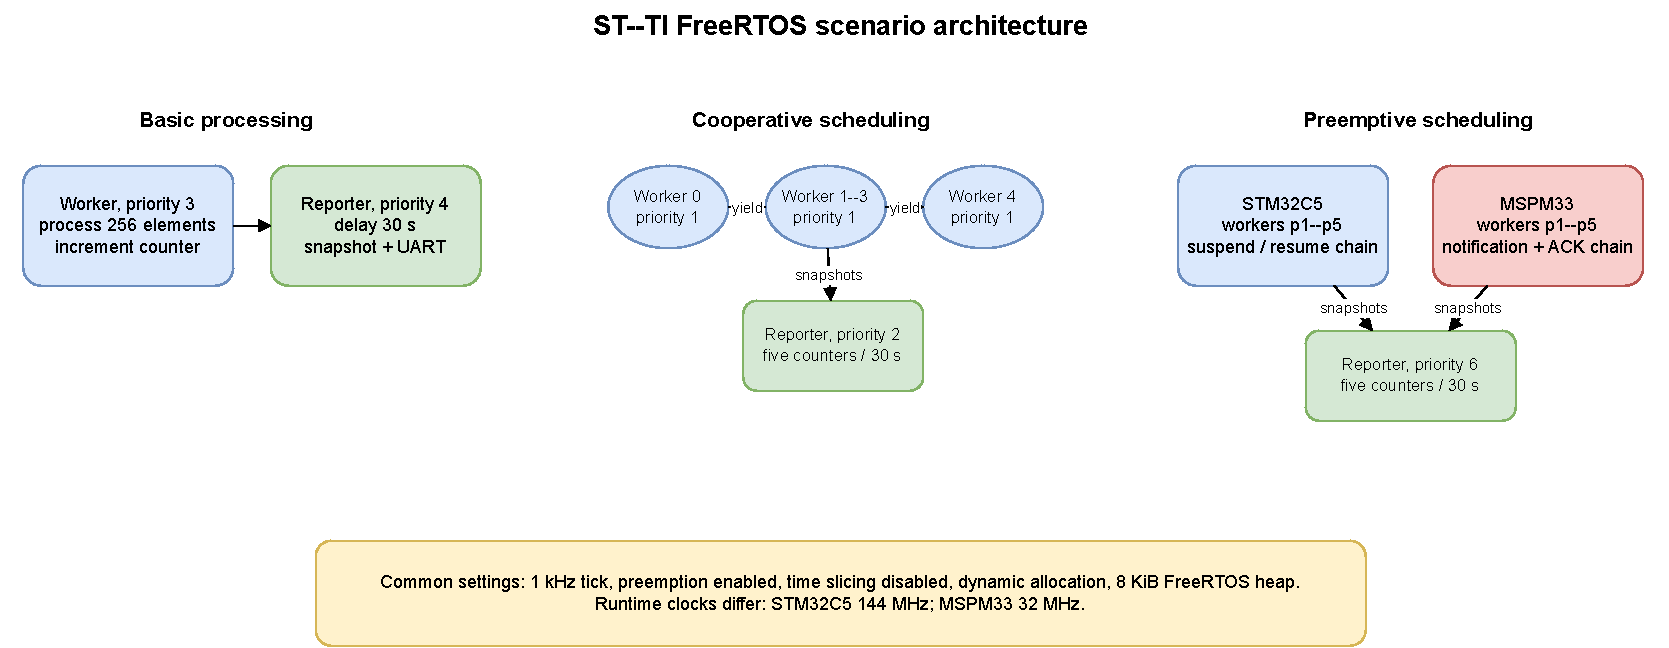
\includegraphics[width=\textwidth]{Figures/ti-freertos/scenario-architecture.pdf}
\caption{Task architecture of the three ST--TI FreeRTOS scenarios. The preemptive scenario deliberately shows the non-equivalent synchronisation paths found in the measured projects.}
\label{fig:ti-freertos-architecture}
\end{figure}

\begin{table}[H]
\centering
\caption{FreeRTOS scenario semantics and reported metric.}
\label{tab:ti-freertos-scenarios}
\begin{tabularx}{\textwidth}{l X X}
\toprule
\textbf{Scenario} & \textbf{Task behaviour} & \textbf{Reported metric} \\
\midrule
Basic & One priority-3 worker transforms a 256-element volatile array and increments a counter; a priority-4 reporter samples it. & Completed processing iterations/s \\
Cooperative & Five priority-1 workers call \texttt{taskYIELD()} and increment separate counters; a priority-2 reporter samples all five. & Mean iterations/thread/s \\
Preemptive & Five workers use priorities 1--5 and a priority-6 reporter. STM32 uses a suspend/resume chain; TI uses task notifications and an acknowledgement. & Mean completed chains/thread/s \\
\bottomrule
\end{tabularx}
\end{table}

The basic and cooperative scenarios preserve the same worker count, creation order, priorities,
and counter semantics on both platforms. The preemptive projects do not preserve the same
synchronisation primitive: STM32 uses \texttt{vTaskSuspend()} and \texttt{vTaskResume()}, while
TI uses direct task notifications plus a final acknowledgement. Its result therefore compares
the two complete implementations but cannot isolate the cost of a common preemption mechanism.

\subsection{Measurement method and fairness}
\label{subsec:ti-freertos-method}

Runtime values were obtained from UART captures supplied after executing both boards. Each row
in Table~\ref{tab:ti-freertos-runtime} is the mean of the available 30-second windows: three
STM32 and two TI windows for basic processing, two and four for cooperative processing, and two
and six for preemptive processing. No warm-up interval or dispersion statistic was recorded.
Cooperative and preemptive reporters advance a nominal time by 30\,s; because UART output occurs
before the next delay, reporting time is outside their denominator.

The largest fairness difference is the configured core clock: STM32C5 runs at 144\,MHz with
instruction cache enabled, whereas MSPM33 runs at 32\,MHz. Both targets use a Cortex-M33 and
Virtual Floating-Point version~5 (VFPv5) single-precision configuration, but the clock ratio is
4.5:1. We therefore report the raw rates and a clock-normalised ratio

\[
R_{\mathrm{norm}} = \frac{R_{\mathrm{STM32}}/144}{R_{\mathrm{MSPM33}}/32}.
\]

A value near one indicates that the raw difference is explained approximately by configured
clock frequency; it is not a direct measurement of cycles per context switch.

\subsection{Results}
\label{subsec:ti-freertos-results}

\begin{table}[H]
\centering
\caption{Observed FreeRTOS runtime rates and clock-normalised STM32/MSPM33 ratio.}
\label{tab:ti-freertos-runtime}
\begin{tabular}{l r r r}
\toprule
\textbf{Scenario} & \textbf{STM32C5 rate} & \textbf{MSPM33 rate} & $\boldsymbol{R_{\mathrm{norm}}}$ \\
\midrule
Basic processing & 43\,172.93 iterations/s & 9\,570.47 iterations/s & 1.002 \\
Cooperative & 226\,652.76 iterations/thread/s & 35\,783.68 iterations/thread/s & 1.408 \\
Preemptive & 55\,015.52 chains/thread/s & 7\,110.96 chains/thread/s & 1.719 \\
\bottomrule
\end{tabular}
\end{table}

\reportscreenshot
      {Figures/ti-freertos/screenshots/uart-runtime-windows.png}
      {Place the STM32C5 and MSPM33 UART captures side by side. Show the board identity, scenario, raw counters, 30-second reporting window, and enough repeated windows to support the values in the runtime table.}
      {Raw UART reporting windows used for the ST--TI FreeRTOS runtime comparison.}
      {fig:ti-screenshot-freertos-uart}

Basic processing scales almost exactly with the configured clock ratio: after normalisation,
STM32C5 and MSPM33 differ by only 0.2\%. The cooperative observation retains a normalised ratio
of 1.408, but this value includes the complete worker loop, FreeRTOS port, compiler runtime,
cache and memory behaviour; it does not measure \texttt{taskYIELD()} in isolation. The
preemptive ratio is larger still, but the different kernel versions and synchronisation
primitives prevent attribution to scheduler efficiency. One TI cooperative run printed
\texttt{ERROR} because the shared integer-truncated balance check allowed only a one-count
deviation; the individual counters remained within the observed scheduling pattern, so this is
treated as a benchmark-check limitation rather than a demonstrated kernel failure.

All six images were rebuilt with IAR EWARM~9.60.3 using high optimisation for size. The
recorded options are \texttt{CCOptLevel=3} and \texttt{CCOptStrategy=1}. Flash is read-only
code plus read-only data; RAM is read-write data, following the linker-map accounting used in
Section~\ref{subsec:ti-functional-results}~\cite{iar-ewarm}.

\begin{table}[H]
\centering
\caption{FreeRTOS whole-image footprint under IAR high/size optimisation (bytes).}
\label{tab:ti-freertos-footprint}
\resizebox{\textwidth}{!}{%
\begin{tabular}{l r r r r r r}
\toprule
& \multicolumn{3}{c}{\textbf{Flash}} & \multicolumn{3}{c}{\textbf{RAM}} \\
\cmidrule(lr){2-4}\cmidrule(lr){5-7}
\textbf{Scenario} & \textbf{STM32} & \textbf{TI} & \textbf{ST--TI} & \textbf{STM32} & \textbf{TI} & \textbf{ST--TI} \\
\midrule
Basic & 9\,052 & 12\,854 & -3\,802 (-29.6\%) & 10\,196 & 10\,140 & +56 (+0.6\%) \\
Cooperative & 9\,640 & 13\,430 & -3\,790 (-28.2\%) & 9\,188 & 9\,132 & +56 (+0.6\%) \\
Preemptive & 10\,012 & 13\,894 & -3\,882 (-27.9\%) & 9\,188 & 9\,112 & +76 (+0.8\%) \\
\midrule
\textbf{Total} & \textbf{28\,704} & \textbf{40\,178} & \textbf{-11\,474 (-28.6\%)} & \textbf{28\,572} & \textbf{28\,384} & \textbf{+188 (+0.7\%)} \\
\bottomrule
\end{tabular}
}
\end{table}

Unlike the low-level-driver portfolio, the middleware result consistently favours STM32C5 in
flash: its three images are 27.9--29.6\% smaller, for an aggregate reduction of 11\,474 bytes.
TI uses slightly less RAM in every scenario, but the difference is only 56--76 bytes per image.
These totals include each platform's complete startup, configuration, C runtime, FreeRTOS
kernel/port, application, heap, and stack reservations. TI links an externally built FreeRTOS
library, while STM32 compiles the kernel sources in each project; configuration also differs in
task notifications, stack-overflow checking, application task tags, and thread-local-storage
pointers. The footprint gap is consequently a result for these deployable SDK configurations,
not a kernel-only size comparison.

Appendix~\ref{sec:appendix-ti-freertos} preserves the raw UART windows, project configuration,
primitive mapping, and linker-map totals used for these calculations.

\subsection{Takeaway}
\label{subsec:ti-freertos-takeaway}

The FreeRTOS benchmark adds two findings to the ST--TI comparison. First, the STM32C5 projects
produce substantially smaller linked flash images while MSPM33 retains a marginal RAM
advantage. Second, raw runtime rates cannot be read as a direct platform ranking: the basic
scenario is almost entirely explained by the 4.5:1 clock ratio, and the more complex scenarios
retain differences that are confounded by kernel configuration and, for preemption, different
synchronisation semantics. A controlled follow-up should use equal clocks, one FreeRTOS version
and configuration, equal primitives, equal sample counts, a warm-up policy, and cycle-level
measurement boundaries.


\newpage
\section*{Conclusion}
This chapter presented the ST-versus-TI comparison of the STM32CubeC5 LL layer and TI
driverlib. The static phase covered seven quality dimensions and an SDK inventory comparison
for the selected releases. The functional phase then mapped twelve bare-metal scenarios spanning ADC, GPIO,
I\textsuperscript{2}C, SPI, and UART behaviour, and documented their observable completion
criteria.

Within the analysed source sets, STM32CubeC5 records higher measured documentation coverage,
lower duplication and average cyclomatic complexity, and a lower adjusted Cppcheck
MISRA-addon finding count. The SDK inventory also identifies broader ST coverage in several
connectivity and security categories. These findings describe the selected SDK versions and
analysis configuration; they do not establish overall ecosystem maturity, certified MISRA
compliance, runtime performance, or product-level software quality.

TI's analysed driverlib makes wider use of enums and typedefs, while the SDK inventory
identifies distinct analog, post-quantum cryptography, AI, graphics, and automotive
capabilities. These are source-structure, datasheet, and inventory observations rather than
measured advantages in execution time, analog performance, safety, or application
suitability.

The functional phase provides whole-image footprint evidence for both the low-level-driver and
FreeRTOS portfolios. The driver scenarios slightly favour MSPM33 in aggregate flash and STM32C5
in RAM, whereas all three FreeRTOS images favour STM32C5 in flash and MSPM33 by a small RAM
margin. Runtime observations are available for FreeRTOS, but unequal clocks, kernel versions,
configuration options, sample counts, and preemptive primitives limit their interpretation.
The basic result is almost exactly clock-proportional; cooperative and preemptive differences
require a controlled follow-up before they can support scheduler-efficiency conclusions.

\chapter*{General Conclusion and Perspectives}
\phantomsection
\addcontentsline{toc}{chapter}{General Conclusion and Perspectives}
\label{chap:cascade-general-conclusion}

This internship produced one standalone product-comparison assignment followed by an
independent sequence of benchmark and tooling contributions. Keeping those workstreams
separate avoids implying a methodological dependency that did not exist.

For the board-equivalence assignment, the host team supplied the competitor-board list and
asked us to identify the nearest STM32 counterparts. The resulting mappings are useful only
when their criteria are stated, particularly where
the paired boards use different Cortex-M architectures or expose different memory,
peripheral, and software environments. The official ST product page confirms that the
``SM32H735G-DK'' spelling in the internal summary refers to
STM32H735G-DK~\cite{st-stm32h735g-dk}. This assignment did not
select or constrain the boards used in the later benchmark chapters.

The independent benchmark work began with the USB pilot. Optimising the STM32H573I-DK reference
reduced RAM and initialisation time in HID, CDC, and MSC, while ROM remained almost
unchanged in two scenarios. In the recorded Renesas comparison, the optimised STM32 project
has lower summary ROM, RAM, and initialisation values than RA6M5 in all three scenarios.
This is an implementation-level result, not a universal vendor ranking.

The NXP pilot exposed a different trade-off. The workbook lists an average STM32 ROM gap
of $+26.22\,\%$ when RCC is included and $+4.16\,\%$ when it is removed. MCX-N9 retains
the lower summary RAM values and lower recorded initialisation values, while the HID ROM
ordering changes with the measurement boundary. The reviewed presentation resolves the
conflicting workbook cells: its tables confirm the reported HID and CDC ROM values and the
MSC RAM values, while its flowchart identifies the timing case as MSC host initialisation.

The manual reconciliation required by these pilots motivated MCU Workflow Studio and the
MCU Benchmark Copilot Agent. The first structures linker-map analysis and cross-vendor
classification; the second assists project preparation, campaign execution, provenance,
and fairness review. Their value lies in formalising and supporting the method. They do not
replace source artifacts, hardware evidence, or engineering judgement.

The later GD32 and TI campaigns broadened the experimental scope. The GD32 work combined
USB and FreeRTOS observations and revealed different flash, RAM, and reported timing
trade-offs rather than a uniform ecosystem advantage. The TI work combined static driver
analysis, matched bare-metal projects, and FreeRTOS scenarios. Across twelve independently
linked bare-metal images, STM32C5 used 2.8\,\% more aggregate flash and 5.0\,\% less
aggregate RAM. In the three FreeRTOS images, STM32C5 used 27.9--29.6\,\% less flash,
whereas MSPM33 retained a 56--76-byte RAM advantage. Unequal clocks and differing kernel
configurations still prevent a scheduler-efficiency conclusion.

\section*{Perspectives}

Runtime experiments should be repeated with documented equal clocks, software versions,
synchronisation primitives, intervals, warm-up policy, and sample counts, with dispersion
reported alongside central values. The internal evidence register should also be completed
with archived map files, project configurations, and hashes for every published result.

Tool validation forms a second workstream. MCU Workflow Studio should be evaluated on a
larger labelled collection of linker maps, while the MCU Benchmark Copilot Agent should be
assessed through recorded campaigns that distinguish successful automation, manual
intervention, and hardware-dependent steps. Finally, the campaign can be extended to new
middleware and vendors only when each addition preserves explicit measurement boundaries
and fairness limitations. These steps would broaden the evidence without weakening the
central rule established by this work: no comparative conclusion should exceed the
measurements and controls that support it.

\appendix


\chapter{Glossary}
\label{chap:glossary}

\textbf{Architectural layer:} A classification of firmware symbols into one of four categories --- application, middleware, low-level driver, or system runtime --- used to attribute memory costs to comparable functional blocks across vendors.\\

\textbf{Board Support Package (BSP):} A set of drivers and configuration files that adapt a vendor's generic HAL to a specific evaluation or development board.\\

\textbf{Context switch:} The process by which an RTOS saves the CPU state of the currently running task and restores the state of the next task to be executed. Context-switch efficiency directly affects multi-threaded throughput.\\

\textbf{Cross-vendor benchmark:} A controlled experiment in which the same workload runs on two vendor platforms under matched and documented conditions. Residual differences in clocks, toolchains, configuration, or scenario logic are reported as fairness limitations.\\

\textbf{Firmware footprint:} The amount of non-volatile (flash/ROM) and volatile (RAM) memory a firmware image occupies once compiled and linked. It is a static measurement taken from the linked binary, not a dynamic runtime observation.\\

\textbf{Linker map:} A text file produced by the linker at the end of the build process. It lists every module and function linked into the final image together with its code size, constant-data size, and variable-data size. It is the primary input to the footprint analysis tool.\\

\textbf{Middleware:} Software libraries that sit between the hardware abstraction layer and the application, providing protocol or service logic (e.g.\ USB device stack, FreeRTOS kernel, FatFS, LwIP).\\

\textbf{Semantic equivalence:} The degree to which two benchmark implementations preserve the observable behaviour relevant to the comparison, including task structure, timing intent, synchronisation, and reporting format. Any unresolved difference is recorded as a fairness limitation.\\

\textbf{Software stack:} A vertical slice of firmware functionality (e.g.\ USB device, FreeRTOS integration) comprising application code, middleware, and hardware drivers, benchmarked as a unit.\\

\textbf{Tick (RTOS):} The periodic timer interrupt that drives the RTOS scheduler. A 1\,ms tick means the scheduler evaluates task readiness every millisecond.\\

\pagebreak

\input{Endmatter/Acronyms}

\chapter{Complementary Code Listings}
\label{chap:complementary-codes}

This appendix provides representative code excerpts that complement the tool and benchmark
descriptions in the main chapters. They illustrate the formats consumed and produced by our
tools and the firmware structure of the benchmark scenarios.

\lstset{style=mystyle}

% ====================================================================
\section{IAR EWARM linker map excerpt}
\label{sec:appendix-linker-map}

Listing~\ref{lst:linker-map} shows an abbreviated IAR EWARM linker map for a USB HID
project. This is the format parsed by MCU Workflow Studio
(Chapter~\ref{chap:footprint-tool}). Each entry lists a module, its read-only code size,
read-only data, and read-write data --- the three quantities from which flash and RAM
footprint are derived.

\begin{lstlisting}[language={}, caption={Abbreviated IAR EWARM linker map (USB HID, STM32U575).}, label={lst:linker-map}]
*******************************************************************************
*** MODULE SUMMARY
***

    Module               ro code  ro data  rw data
    ------               -------  -------  -------
    main.o                   164       --       --
    stm32u5xx_hal.o          212       --        4
    stm32u5xx_hal_gpio.o     456       --       --
    stm32u5xx_hal_rcc.o    4 560       16       --
    stm32u5xx_hal_pcd.o    2 496       --       --
    stm32u5xx_ll_usb.o     2 492       --       --
    usbd_core.o            1 048       --       --
    usbd_ctlreq.o            876       --       --
    usbd_hid.o               620       --       --
    usbd_conf.o              524       --       32
    usbd_desc.o              461      268       --
    system_stm32u5xx.o       128       16        4
    startup_stm32u575xx.o    394      512       --
    ------               -------  -------  -------
    Total:               14 431      812       40

*******************************************************************************
*** ENTRY LIST
***

    Entry                 Address    Size  Type  Object
    -----                 -------    ----  ----  ------
    HAL_Init             0x0800'1234   52  Code  stm32u5xx_hal.o
    HAL_RCC_OscConfig    0x0800'2000  1024  Code  stm32u5xx_hal_rcc.o
    HAL_RCC_ClockConfig  0x0800'2400   896  Code  stm32u5xx_hal_rcc.o
    USBD_Init            0x0800'3000   128  Code  usbd_core.o
    USBD_HID_Init        0x0800'3200    96  Code  usbd_hid.o
    ...
\end{lstlisting}

\pagebreak

% ====================================================================
\section{ST--TI functional footprint reproducibility record}
\label{sec:appendix-ti-functional-footprint}

This appendix records the build and accounting conditions behind the ST-versus-TI functional
footprint results in Chapter~\ref{chap:vs-ti}. The TI projects are MSPM33 SDK driverlib
examples~\cite{ti-mspm33-sdk}; their counterparts are STM32CubeC5 LL examples~\cite{stm32cubec5-sw}.
All twelve pairs were rebuilt with IAR EWARM~9.60.3 using high optimisation for size
(\texttt{CCOptLevel=3}, \texttt{CCOptStrategy=1}). The IAR linker map reports read-only code,
read-only data, and read-write data~\cite{iar-ewarm}. We use the following whole-image accounting:

\[
\text{Flash} = \text{RO code} + \text{RO data}, \qquad
\text{RAM} = \text{RW data}.
\]

Both projects in every pair reserve a 512-byte stack in the linker map. The table is therefore
reproducible from the matching IAR map files and includes the deployable image's startup and
vector-table cost. It is a portfolio of independent images, not the footprint of one firmware
that combines all scenarios.

\begin{table}[H]
\centering
\scriptsize
\caption{Reproducibility record for the ST--MSPM33 high/size functional footprint study (bytes).}
\label{tab:appendix-ti-functional-footprint}
\resizebox{\textwidth}{!}{%
\begin{tabular}{l r r r r r r}
\toprule
\textbf{Scenario} & \textbf{MSPM33 flash} & \textbf{STM32 flash} & \textbf{Delta} & \textbf{MSPM33 RAM} & \textbf{STM32 RAM} & \textbf{Delta} \\
\midrule
ADC timer trigger & 1\,476 & 1\,416 & -60 & 513 & 513 & 0 \\
GPIO toggle & 656 & 772 & +116 & 512 & 512 & 0 \\
I\textsuperscript{2}C DMA controller & 1\,928 & 1\,840 & -88 & 553 & 517 & -36 \\
I\textsuperscript{2}C DMA responder & 1\,744 & 1\,687 & -57 & 593 & 556 & -37 \\
I\textsuperscript{2}C interrupt controller & 1\,580 & 1\,732 & +152 & 557 & 514 & -43 \\
I\textsuperscript{2}C interrupt responder & 1\,388 & 1\,460 & +72 & 600 & 553 & -47 \\
I\textsuperscript{2}C polling controller & 1\,420 & 1\,376 & -44 & 556 & 513 & -43 \\
I\textsuperscript{2}C polling responder & 1\,412 & 1\,340 & -72 & 608 & 552 & -56 \\
SPI DMA controller & 1\,704 & 2\,151 & +447 & 592 & 556 & -36 \\
SPI DMA peripheral & 1\,876 & 1\,940 & +64 & 592 & 552 & -40 \\
UART printf & 1\,326 & 1\,318 & -8 & 512 & 512 & 0 \\
USART loopback & 1\,588 & 1\,580 & -8 & 532 & 532 & 0 \\
\midrule
\textbf{Total, 12 independent images} & \textbf{18\,098} & \textbf{18\,612} & \textbf{+514} & \textbf{6\,720} & \textbf{6\,382} & \textbf{-338} \\
\bottomrule
\end{tabular}%
}
\end{table}

Negative deltas favour STM32C5. The corresponding interpretation, fairness limits, and
scenario-flow diagrams are presented in Section~\ref{sec:ti-functional-analysis}; this appendix
is intentionally limited to reproducibility facts and raw whole-image totals.

\pagebreak

% ====================================================================
\section{ST--TI FreeRTOS reproducibility record}
\label{sec:appendix-ti-freertos}

The FreeRTOS middleware benchmark in Section~\ref{sec:ti-freertos} uses three matched project
pairs from STM32CubeC5 and MSPM33 SDK~1.04.00.00~\cite{stm32cubec5-sw,ti-mspm33-sdk}. All six
images were built with IAR EWARM~9.60.3 at high optimisation for size
(\texttt{CCOptLevel=3}, \texttt{CCOptStrategy=1})~\cite{iar-ewarm}. The common configuration
includes a 1\,kHz tick, preemption enabled, time slicing disabled, dynamic allocation, ten
priorities, and an 8\,KiB FreeRTOS heap. STM32C5 was configured at 144\,MHz and MSPM33 at
32\,MHz; these are source configuration values rather than independent clock measurements.
Project manifests identify FreeRTOS Kernel~V11.2.0 for STM32C5 and V11.1.0 for MSPM33. In the
preemptive scenario, STM32 uses \texttt{vTaskSuspend()}/\texttt{vTaskResume()}, whereas MSPM33
uses direct task notifications and a final acknowledgement.

\begin{table}[H]
\centering
\caption{Raw UART observation windows for the ST--TI FreeRTOS benchmark.}
\label{tab:appendix-ti-freertos-runtime}
\small
\begin{tabularx}{\textwidth}{l l X}
\toprule
\textbf{Scenario} & \textbf{Platform} & \textbf{Recorded 30-second deltas} \\
\midrule
Basic & STM32C5 & 1\,295\,358; 1\,295\,330; 1\,295\,351. Elapsed: 30\,000; 30\,005; 30\,006\,ms. \\
Basic & MSPM33 & 287\,141; 287\,135. Elapsed: 30\,000; 30\,005\,ms. \\
Cooperative & STM32C5 & 33\,998\,170; 33\,997\,657 total worker iterations \\
Cooperative & MSPM33 & 5\,367\,603; 5\,367\,557; 5\,367\,559; 5\,367\,490 total worker iterations \\
Preemptive & STM32C5 & 8\,252\,379; 8\,252\,277 total completed chains \\
Preemptive & MSPM33 & 1\,066\,661; 1\,066\,639; 1\,066\,639; 1\,066\,637; 1\,066\,635; 1\,066\,655 total completed chains \\
\bottomrule
\end{tabularx}
\end{table}

\begin{table}[H]
\centering
\caption{IAR high/size map totals for the ST--TI FreeRTOS projects (bytes).}
\label{tab:appendix-ti-freertos-footprint}
\begin{tabular}{l r r r r}
\toprule
\textbf{Scenario} & \textbf{STM32 flash} & \textbf{MSPM33 flash} & \textbf{STM32 RAM} & \textbf{MSPM33 RAM} \\
\midrule
Basic & 9\,052 & 12\,854 & 10\,196 & 10\,140 \\
Cooperative & 9\,640 & 13\,430 & 9\,188 & 9\,132 \\
Preemptive & 10\,012 & 13\,894 & 9\,188 & 9\,112 \\
\midrule
\textbf{Total} & \textbf{28\,704} & \textbf{40\,178} & \textbf{28\,572} & \textbf{28\,384} \\
\bottomrule
\end{tabular}
\end{table}

The runtime record is not a controlled equal-clock experiment. Sample counts differ, no
warm-up policy is documented, and the preemptive implementations use different synchronisation
primitives. The tables preserve the raw evidence so that later equal-clock measurements can be
compared without replacing or silently reinterpreting the original observations.

\pagebreak

% ====================================================================
\section{Agent configuration file}
\label{sec:appendix-agent-config}

Listing~\ref{lst:agent-config} shows the configuration of the Creation-Porting specialist
agent from the MCU Benchmark Copilot Agent system
(Chapter~\ref{chap:benchmark-agent}). The YAML frontmatter declares metadata, description,
argument hints, and tool permissions; the Markdown body contains the behavioural
instructions, autonomy contract, and supported workflow directions.

\begin{lstlisting}[language={}, caption={Creation-Porting agent configuration (abbreviated).}, label={lst:agent-config}]
---
name: Creation-Porting
description: "Create benchmark projects from scratch or port existing
  benchmarks in any direction (STM32->competitor, competitor->STM32,
  vendor->vendor, board->board). Use when: generating target project
  files, creating from a scenario description, separating
  portable/RTOS/board logic, or acquiring missing reference firmware."
argument-hint: A benchmark requirement, scenario description, scenario
  name, firmware name, or a reference project plus target platform.
tools: ['read', 'search', 'edit', 'vscode', 'todo', 'web', 'execute']
---

# Creation-Porting Agent

## Supported Directions
- From scratch (scenario description only)
- STM32 -> competitor
- Competitor -> STM32
- Vendor A -> Vendor B
- Board A -> Board B
- Name only (resolve, acquire, create)

## Autonomy Contract
- Operates autonomously for file generation, project creation, and
  material acquisition (web fetches from official sources).
- Asks only before flashing/programming/resetting hardware.
- Acquires missing firmware, CMSIS, BSP, startup, linker from
  official vendor GitHub repos and SDKs without confirmation.

## IAR Template Resolution
Before creating any project:
1. Look up target board in config/iar_templates.yaml
2. Follow resolution: exact board -> family fallback -> type fallback
3. Acquire template if status == "needs_download"
4. Use materialised template as read-only project baseline
5. Place benchmark code through app_integration_points only

## Multi-Layer Separation
1. Portable application layer (writable) - benchmark logic
2. RTOS / middleware layer (protected) - select, don't modify
3. Board-specific layer (protected) - select existing vendor files
4. Build surface (configure only) - .ewp references, defines, paths

## Semantic Preservation Rule
Preserve semantics and observable behaviors, not vendor API names.
Map CMSIS-RTOS2 <-> native FreeRTOS <-> ThreadX as needed via
app-level adapter files. Never modify vendor HAL source.
\end{lstlisting}

\pagebreak

% ====================================================================
\section{FreeRTOS cooperative benchmark scenario}
\label{sec:appendix-freertos-coop}

Listing~\ref{lst:freertos-coop} shows the core task logic of the cooperative processing
benchmark scenario from Chapter~\ref{chap:vs-gd32}. Five equal-priority threads each
increment a counter and yield; a reporter thread prints the results every 30~seconds.

\begin{lstlisting}[language=C, caption={FreeRTOS cooperative scenario --- task functions (STM32, simplified).}, label={lst:freertos-coop}]
/* Shared counters for the five worker threads */
volatile uint32_t counters[5] = {0};

/* Worker task: increment own counter, then yield */
void WorkerTask(void *param)
{
    uint32_t id = (uint32_t)param;
    for (;;)
    {
        counters[id]++;
        taskYIELD();
    }
}

/* Reporter task: print all counters every 30 s */
void ReporterTask(void *param)
{
    (void)param;
    for (;;)
    {
        vTaskDelay(pdMS_TO_TICKS(30000));
        printf("Counters: %lu %lu %lu %lu %lu\r\n",
               counters[0], counters[1], counters[2],
               counters[3], counters[4]);
        /* Reset for next interval */
        for (int i = 0; i < 5; i++)
            counters[i] = 0;
    }
}

/* Task creation (in main, after HAL and kernel init) */
void CreateBenchmarkTasks(void)
{
    for (uint32_t i = 0; i < 5; i++)
    {
        xTaskCreate(WorkerTask, "Worker", 128,
                    (void *)i, tskIDLE_PRIORITY + 1, NULL);
    }
    xTaskCreate(ReporterTask, "Reporter", 256,
                NULL, tskIDLE_PRIORITY + 2, NULL);
    vTaskStartScheduler();
}
\end{lstlisting}

\pagebreak

% ====================================================================
\section{Footprint tool CLI output}
\label{sec:appendix-tool-output}

Listing~\ref{lst:tool-output} shows a representative terminal output from a footprint
benchmark run using the MCU Workflow Studio command-line interface
(Chapter~\ref{chap:footprint-tool}).

\begin{lstlisting}[language={}, caption={MCU Workflow Studio CLI --- benchmark summary output.}, label={lst:tool-output}]
$ mcu-workflow-cli benchmark \
    --source stm32_usb_hid.map --source-vendor stm32 \
    --target gd32_usb_hid.map  --target-vendor gd32 \
    --out results/

[INFO] Parsing source map: stm32_usb_hid.map (IAR EWARM)
[INFO] Parsing target map: gd32_usb_hid.map (IAR EWARM)
[INFO] Classifying 47 source symbols into layers...
[INFO] Classifying 31 target symbols into layers...
[INFO] Mapping engine: 42 pairs scored, 38 accepted (confidence >= 0.72)
[INFO] 4 pairs queued for review (confidence 0.55-0.72)

=== FOOTPRINT COMPARISON (USB HID) ===

Layer           | STM32 ROM | GD32 ROM  | Diff
----------------|-----------|-----------|--------
Application     |   2 580 B |   1 942 B | +33%
HAL drivers     |  10 426 B |     820 B | +1171%
MW stack        |   2 859 B |   5 743 B | -50%
----------------|-----------|-----------|--------
TOTAL ROM       |  16 269 B |   9 175 B | +77%
TOTAL RAM       |   3 446 B |   9 608 B | -65%

Verdict: STM32 uses +77% more ROM but -65% less RAM.
Largest classified STM32 modules:
    HAL RCC:       4560 B
    HAL/LL USB:    4988 B
Causal attribution: unresolved without complete maps and classification diagnostics.

[INFO] Results written to results/benchmark_results.xlsx
[INFO] Mapping diagnostics: results/mapping_diagnostics.json
[INFO] Review queue (4 items): results/review_queue.csv
\end{lstlisting}

\pagebreak

% ====================================================================
\section{Static-analysis automation script (ST vs.\ TI)}
\label{sec:appendix-analyze-firmware}

Listing~\ref{lst:analyze-firmware} shows an abbreviated version of the Python script used
to extract API surface and documentation coverage metrics for the ST-versus-TI static
analysis (Chapter~\ref{chap:vs-ti}). The full script analyses duplication, documentation,
and API design in a single pass over the driver source trees.

\begin{lstlisting}[language=Python, caption={Abbreviated \texttt{analyze\_firmware.py} --- API and documentation extraction.}, label={lst:analyze-firmware}]
"""
Firmware benchmark analysis script:
- Code duplication detection (sliding-window hash)
- Documentation coverage (Doxygen tag extraction)
- API surface area analysis (functions, macros, enums)
"""
import os, re, json, hashlib
from collections import defaultdict, Counter
from pathlib import Path

TI_DIR = r"mspm33_sdk/source/ti/driverlib"
ST_DIR = r"STM32CubeC5/stm32c5xx_drivers/ll"

def get_c_files(directory):
    files = []
    for root, _, filenames in os.walk(directory):
        for f in filenames:
            if f.endswith(('.c', '.h')):
                files.append(os.path.join(root, f))
    return files

def analyze_api(files):
    """Extract API surface metrics from C source files."""
    result = {
        'public_functions': 0, 'static_functions': 0,
        'inline_functions': 0, 'macros_functional': 0,
        'macros_constant': 0, 'enums': 0, 'typedefs': 0,
        'param_distribution': Counter(),
    }
    for filepath in files:
        with open(filepath, 'r', errors='ignore') as f:
            content = f.read()
        # Count public functions (not static)
        pub = re.findall(
            r'(?<!static\s)(?:__STATIC_INLINE\s+|inline\s+)?'
            r'(?:void|bool|uint\w+|int\w+|DL_\w+|LL_\w+)\s+'
            r'(\w+)\s*\(([^)]*)\)', content)
        for name, params in pub:
            result['public_functions'] += 1
            n = len([p for p in params.split(',')
                     if p.strip()]) if params.strip() else 0
            result['param_distribution'][n] += 1
        # Count enums, typedefs, macros
        result['enums'] += len(re.findall(
            r'\benum\s+\w*\s*\{', content))
        result['typedefs'] += len(re.findall(
            r'\btypedef\s+', content))
        result['macros_functional'] += len(re.findall(
            r'#define\s+\w+\([^)]*\)', content))
        result['macros_constant'] += len(re.findall(
            r'#define\s+\w+\s+[^(]', content))
    return result

if __name__ == '__main__':
    for label, path in [("TI", TI_DIR), ("ST", ST_DIR)]:
        files = get_c_files(path)
        api = analyze_api(files)
        print(f"\n=== {label} API Surface ===")
        for k, v in api.items():
            print(f"  {k}: {v}")
\end{lstlisting}


\begin{thebibliography}{99}
\addcontentsline{toc}{chapter}{Bibliography}

% --- References cited in Chapter~\ref{chap:general-description} ---

\bibitem{st-about}
STMicroelectronics, \emph{About ST}. [Online]. Available: \url{https://www.st.com/content/st_com/en/about/st_company_information.html}. Accessed: 2026.

\bibitem{st-investors}
STMicroelectronics, \emph{2024 Annual Report and Financial Highlights}. [Online]. Available: \url{https://investors.st.com/}. Accessed: 2026.

\bibitem{st-strategy}
STMicroelectronics, \emph{Strategy and Innovation}. [Online]. Available: \url{https://www.st.com/content/st_com/en/about/innovation---technology/innovation---technology.html}. Accessed: 2026.

\bibitem{stm32-family}
STMicroelectronics, \emph{STM32 32-bit Arm Cortex MCUs}. [Online]. Available: \url{https://www.st.com/en/microcontrollers-microprocessors/stm32-32-bit-arm-cortex-mcus.html}. Accessed: 2026.

\bibitem{arm-cortexm}
Arm Ltd., \emph{Cortex-M Series Processors}. [Online]. Available: \url{https://developer.arm.com/Processors/Cortex-M}. Accessed: 2026.

\bibitem{stm32cube-ecosystem}
STMicroelectronics, \emph{STM32Cube Ecosystem}. [Online]. Available: \url{https://www.st.com/en/ecosystems/stm32cube.html}. Accessed: 2026.

\bibitem{divide-conquer}
T.~H. Cormen, C.~E. Leiserson, R.~L. Rivest, and C.~Stein, \emph{Introduction to Algorithms}, 3rd~ed. Cambridge, MA: MIT Press, 2009.

% --- Official product sources for the standalone board-equivalence assignment ---

\bibitem{nxp-imxrt1060-evk}
NXP Semiconductors, \emph{i.MX RT1060 Evaluation Kit}. [Online]. Available: \url{https://www.nxp.com/design/design-center/development-boards-and-designs/MIMXRT1060-EVKB}. Accessed: 2026-08-24.

\bibitem{st-stm32h735g-dk}
STMicroelectronics, \emph{STM32H735G-DK Discovery Kit with STM32H735IG MCU}. [Online]. Available: \url{https://www.st.com/en/evaluation-tools/stm32h735g-dk.html}. Accessed: 2026-08-24.

\bibitem{nxp-frdm-mcxa156}
NXP Semiconductors, \emph{FRDM Development Board for MCX A144/5/6 and A154/5/6 MCUs}. [Online]. Available: \url{https://www.nxp.com/design/design-center/development-boards-and-designs/FRDM-MCXA156}. Accessed: 2026-08-24.

\bibitem{st-nucleo-l552ze-q}
STMicroelectronics, \emph{NUCLEO-L552ZE-Q: STM32 Nucleo-144 Development Board with STM32L552ZE MCU}. [Online]. Available: \url{https://www.st.com/en/evaluation-tools/nucleo-l552ze-q.html}. Accessed: 2026-08-24.

\bibitem{renesas-fpb-ra0e1}
Renesas Electronics Corporation, \emph{FPB-RA0E1: RA0E1 Fast Prototyping Board}. [Online]. Available: \url{https://www.renesas.com/en/design-resources/boards-kits/fpb-ra0e1}. Accessed: 2026-08-24.

\bibitem{st-nucleo-l031k6}
STMicroelectronics, \emph{NUCLEO-L031K6: STM32 Nucleo-32 Development Board with STM32L031K6 MCU}. [Online]. Available: \url{https://www.st.com/en/evaluation-tools/nucleo-l031k6.html}. Accessed: 2026-08-24.

\bibitem{renesas-fpb-ra8e1}
Renesas Electronics Corporation, \emph{FPB-RA8E1: Fast Prototyping Board for RA8E1 MCU Group}. [Online]. Available: \url{https://www.renesas.com/en/design-resources/boards-kits/fpb-ra8e1}. Accessed: 2026-08-24.

\bibitem{st-nucleo-h743zi2}
STMicroelectronics, \emph{NUCLEO-H743ZI and NUCLEO-H743ZI2 STM32 Nucleo-144 Development Boards}. [Online]. Available: \url{https://www.st.com/en/evaluation-tools/nucleo-h743zi.html}. Accessed: 2026-08-24.

\bibitem{ti-lp-mspm0c1104}
Texas Instruments, \emph{LP-MSPM0C1104: MSPM0C1104 LaunchPad Development Kit for 24-MHz Arm Cortex-M0+ MCU}. [Online]. Available: \url{https://www.ti.com/tool/LP-MSPM0C1104}. Accessed: 2026-08-24.

\bibitem{st-nucleo-f429zi}
STMicroelectronics, \emph{NUCLEO-F429ZI: STM32 Nucleo-144 Development Board with STM32F429ZI MCU}. [Online]. Available: \url{https://www.st.com/en/evaluation-tools/nucleo-f429zi.html}. Accessed: 2026-08-24.

% --- External tools, libraries, and references cited in Chapter~\ref{chap:footprint-tool} ---

\bibitem{python}
Python Software Foundation, \emph{The Python Language Reference, version~3.11}. [Online]. Available: \url{https://docs.python.org/3.11/}. Accessed: 2026.

\bibitem{pyside6}
The Qt Company, \emph{Qt for Python (PySide6) Documentation}. [Online]. Available: \url{https://doc.qt.io/qtforpython/}. Accessed: 2026.

\bibitem{pandas}
The pandas development team, \emph{pandas: Powerful Python Data Analysis Toolkit}. [Online]. Available: \url{https://pandas.pydata.org/}. Accessed: 2026.

\bibitem{openpyxl}
E.~Gazoni and C.~Clark, \emph{openpyxl: A Python Library to Read and Write Excel 2010 xlsx/xlsm Files}. [Online]. Available: \url{https://openpyxl.readthedocs.io/}. Accessed: 2026.

\bibitem{matplotlib}
J.~D. Hunter, ``Matplotlib: A 2D Graphics Environment,'' \emph{Computing in Science \& Engineering}, vol.~9, no.~3, pp.~90--95, 2007. [Online]. Available: \url{https://matplotlib.org/}. Accessed: 2026-08-24.

\bibitem{sqlite}
SQLite Development Team, \emph{SQLite Documentation}. [Online]. Available: \url{https://www.sqlite.org/docs.html}. Accessed: 2026.

\bibitem{pyinstaller}
PyInstaller Development Team, \emph{PyInstaller Manual}. [Online]. Available: \url{https://pyinstaller.org/}. Accessed: 2026.

\bibitem{iar-ewarm}
IAR Systems, \emph{IAR Embedded Workbench for Arm --- C/C++ Development Guide (ILINK Linker and Linker Map File)}. [Online]. Available: \url{https://www.iar.com/embedded-development-tools/iar-embedded-workbench}. Accessed: 2026.

\bibitem{github-copilot}
GitHub, \emph{GitHub Copilot Documentation}. [Online]. Available: \url{https://docs.github.com/en/copilot}. Accessed: 2026.

\bibitem{anthropic}
Anthropic, \emph{Claude API Documentation}. [Online]. Available: \url{https://docs.anthropic.com/}. Accessed: 2026.

\bibitem{openai-api}
OpenAI, \emph{OpenAI API Reference}. [Online]. Available: \url{https://platform.openai.com/docs/}. Accessed: 2026.

\bibitem{ollama}
Ollama, \emph{Ollama: Run Large Language Models Locally}. [Online]. Available: \url{https://ollama.com/}. Accessed: 2026.

\bibitem{github-models}
GitHub, \emph{GitHub Models Documentation}. [Online]. Available: \url{https://docs.github.com/en/github-models}. Accessed: 2026.

\bibitem{nxp-mcuxpresso}
NXP Semiconductors, \emph{MCUXpresso SDK Documentation}. [Online]. Available: \url{https://mcuxpresso.nxp.com/}. Accessed: 2026.

% --- External tools and references cited in Chapter~\ref{chap:benchmark-agent} ---

\bibitem{vscode}
Microsoft, \emph{Visual Studio Code Documentation}. [Online]. Available: \url{https://code.visualstudio.com/docs}. Accessed: 2026.

\bibitem{vscode-agent-mode}
Microsoft, \emph{GitHub Copilot Agent Mode in VS Code}. [Online]. Available: \url{https://code.visualstudio.com/docs/copilot/chat/chat-agent-mode}. Accessed: 2026.

\bibitem{vscode-custom-agents}
Microsoft, \emph{Custom Chat Agents and Skills --- VS Code Documentation}. [Online]. Available: \url{https://code.visualstudio.com/docs/copilot/copilot-customization}. Accessed: 2026.

\bibitem{iar-cspybat}
IAR Systems, \emph{C-SPY Debugging Guide --- Batch Mode (cspybat)}. [Online]. Available: \url{https://www.iar.com/knowledge/support/technical-notes/debugger/}. Accessed: 2026.

% --- References cited in Chapter~\ref{chap:vs-gd32} ---

\bibitem{gigadevice-gd32}
GigaDevice Semiconductor, \emph{GD32 Microcontrollers}. [Online]. Available: \url{https://www.gigadevice.com/microcontroller}. Accessed: 2026.

\bibitem{gd32e507-ds}
GigaDevice Semiconductor, \emph{GD32E507xx Datasheet}, Rev.~1.2, 2022. [Online]. Available: \url{https://www.gigadevice.com/microcontroller/gd32e507zet6}. Accessed: 2026.

\bibitem{stm32u575-ds}
STMicroelectronics, \emph{STM32U575/585 Datasheet --- Ultra-low-power with FPU Arm Cortex-M33 MCU}. [Online]. Available: \url{https://www.st.com/resource/en/datasheet/stm32u575zi.pdf}. Accessed: 2026.

\bibitem{freertos}
Amazon Web Services, \emph{FreeRTOS --- Real-Time Operating System for Microcontrollers}. [Online]. Available: \url{https://www.freertos.org/}. Accessed: 2026.

\bibitem{freertos-v11}
Amazon Web Services, \emph{FreeRTOS V11.2.0 Release Notes}. [Online]. Available: \url{https://github.com/FreeRTOS/FreeRTOS-Kernel/releases/tag/V11.2.0}. Accessed: 2026.

% --- References cited in Chapter~\ref{chap:vs-ti} ---

\bibitem{ti-about}
Texas Instruments, \emph{About TI}. [Online]. Available: \url{https://www.ti.com/about-ti/company/company-overview.html}. Accessed: 2026.

\bibitem{ti-mspm33-product}
Texas Instruments, \emph{MSPM33C321A Product Page}. [Online]. Available: \url{https://www.ti.com/product/MSPM33C321A}. Accessed: 2026.

\bibitem{ti-mspm33-ds}
Texas Instruments, \emph{MSPM33C321A Datasheet}. [Online]. Available: \url{https://www.ti.com/document-viewer/MSPM33C321A/datasheet}. Accessed: 2026.

\bibitem{ti-mspm33-sdk}
Texas Instruments, \emph{MSPM33-SDK --- Software Development Kit for MSPM33}. [Online]. Available: \url{https://www.ti.com/tool/MSPM33-SDK}. Accessed: 2026.

\bibitem{ti-launchpad}
Texas Instruments, \emph{LP-MSPM33C321A LaunchPad Development Kit}. [Online]. Available: \url{https://www.ti.com/tool/LP-MSPM33C321A}. Accessed: 2026.

\bibitem{stm32cubec5-sw}
STMicroelectronics, \emph{STM32CubeC5 --- STM32Cube MCU Package for STM32C5 Series}. [Online]. Available: \url{https://www.st.com/en/embedded-software/stm32cubec5.html}. Accessed: 2026.

\bibitem{stm32c5a3-product}
STMicroelectronics, \emph{STM32C5A3ZG Product Page}. [Online]. Available: \url{https://www.st.com/en/microcontrollers-microprocessors/stm32c5a3zg.html}. Accessed: 2026.

\bibitem{stm32-nucleo-c5a3}
STMicroelectronics, \emph{NUCLEO-C5A3ZG Evaluation Board}. [Online]. Available: \url{https://www.st.com/en/evaluation-tools/nucleo-c5a3zg.html}. Accessed: 2026.

\bibitem{cloc-tool}
A.~Danial, \emph{cloc --- Count Lines of Code}, version~2.08. [Online]. Available: \url{https://github.com/AlDanial/cloc}. Accessed: 2026.

\bibitem{cppcheck-tool}
D.~Marjam\"{a}ki \emph{et~al.}, \emph{Cppcheck --- A Static Analysis Tool for C/C++ Code}. [Online]. Available: \url{https://cppcheck.sourceforge.io/}. Accessed: 2026.

\bibitem{lizard-tool}
T.~Yin, \emph{Lizard --- A Code Complexity Analyser}. [Online]. Available: \url{https://github.com/terryyin/lizard}. Accessed: 2026.

\bibitem{jscpd-tool}
K.~Kravets, \emph{jscpd --- Copy/Paste Detector for Source Code}. [Online]. Available: \url{https://github.com/kucherenko/jscpd}. Accessed: 2026.

\bibitem{misra-c2012}
MISRA, \emph{MISRA C:2012 --- Guidelines for the Use of the C Language in Critical Systems}, 3rd~ed. Nuneaton, UK: MIRA Ltd., 2019.

\bibitem{nist-pqc}
National Institute of Standards and Technology, \emph{Post-Quantum Cryptography Standardization}. [Online]. Available: \url{https://csrc.nist.gov/projects/post-quantum-cryptography}. Accessed: 2026.

\end{thebibliography}

\end{document}